\chapter{The intonation of questions and contrastive focus in Tashlhiyt}
\section{Introduction}
Cross-linguistically, the flagging of questions and the marking of contrastive elements represent communicative functions that are prototypically expressed by means of morphosyntactic devices such as word order or morphological marking. In addition to morphosyntax, these functions can be expressed via prosodic structure and/or intonation. The present chapter will investigate the intonational marking of questions and contrastive statements in Tashlhiyt. We will show that under certain circumstances, both functions are expressed by similar phonetic parameters: questions and contrastive statements are characterised by a rise-fall in pitch. However, even though the pitch movements are very similar in some contexts, there are clear distributional properties and acoustic correlates that systematically distinguish the tonal events in questions from the ones in contrastive statements.\is{focus}

The chapter is structured as follows. After a brief introduction to linguistic aspects of flagging questions and marking contrastive elements (\sectref{sec:5.2}), common cross-linguistic strategies employed to express these functions prosodically and intonationally will be discussed (\sectref{sec:5.3}). Morphosyntactic constructions and the intonational expression of flagging questions and marking contrastive elements in Tashlhiyt are then described based on qualitative observations (\sectref{sec:5.4}). Subsequently, a production study will be presented that provides evidence for both global pitch parameters and local tonal events being used to distinguish questions from corresponding contrastive statements. Moreover, evidence will be presented that the location of tonal events is determined by several interacting factors (\sectref{sec:5.5}). A perception study will be presented that demonstrates the perceptual relevance of the identified cues (\sectref{sec:5.6}).

\section{Theoretical background: questions and focus}\label{sec:5.2}
\subsection{Questions: a working definition}
The distinction between questions and statements is usually defined by a bundle of properties associated with different linguistic levels of description. As a result, the term ‘question’ is used ambiguously in the literature. First, question can refer to a syntactically defined interrogative structure, irrespective of its pragmatic function. An example is the English\il{English} yes-no question which is morphosyntactically distinguished from a corresponding statement by auxiliary fronting (cf. \ref{ex:5:1} and \ref{ex:5:2} below). Second, the term question can also refer to an utterance that functions as a request for information, regardless of its morphosyntactic form. An example is the declarative question in English, which exhibits a declarative syntactic structure (e.g. (\ref{ex:5:3}b) below). Following \citet{Bartels1999} (after \citealt{Lyons1977}, and \citealt{Jacobs1991}), the term ‘question’ shall be used here as a purely functional term referring to utterances that “convey perceived relative lack of information […] regarding a relevant aspect of propositional content” (\citealt[9]{Bartels1999}). In turn, statements are defined as utterances that lack such speaker uncertainty. The following study is limited to two question types: yes-no questions and declarative questions.\is{focus}\is{yes-no question}\is{echo question}

One of the most common and most often discussed question types is the ‘yes-no question’ (henceforth: y/n question, also known as ‘polar question’). It is considered the most basic question type and a near universal across languages (\citealt{SadockZwicky1985}). Compared to a corresponding statement (cf. \ref{ex:5:1}), y/n questions in English can be marked by auxiliary fronting (cf. \ref{ex:5:1} and \ref{ex:5:2}).

\begin{exe}
\ex\label{ex:5:1} Helen ate the chocolate.
\ex\label{ex:5:2} Did Helen eat the chocolate?
\ex\label{ex:5:3} 
\begin{xlist}
                \ex\label{ex:5:3a} I ate the chocolate.
                \ex\label{ex:5:3b} You ate the chocolate?
\end{xlist}
\end{exe} 

Another closely related type of question is the declarative question. This question type is morphosyntactically identical to corresponding statements and is often reported to be distinguished from statements by intonation only (\citealt{Haeseryn.etal1997}). Henceforth the term declarative question will be used to refer to requests for information with declarative syntactic structure. This includes both declarative questions and echo questions. The latter are repetitions of either an entire preceding utterance or parts of it, and express either surprise, disbelief or lack of comprehension, indicating that the proposition the question refers to is unexpected or inappropriate. Echo questions often ask for confirmation or clarification, and can be described as having a bias towards a negative response (cf.~\ref{ex:5:3}).\footnote{Another common question type is the wh-question, which will be briefly discussed in Chapter 7 (see \citealt{Bruggeman.etal2017}, for a first exploration of wh-questions in Tashlhiyt).}\is{yes-no question}\is{echo question}

\subsection{Focus: a working definition}
A pragmatic notion which is orthogonal to the distinction between questions and statements and which is cross-linguistically frequently expressed by intonation is ‘focus’. \citet{Krifka2008} defines focus as the marking of elements to indicate that alternatives to these elements are relevant for the interpretation of the utterance. Consider examples \REF{ex:5:4} and \REF{ex:5:5}.

\begin{exe}
\ex\label{ex:5:4} Helen ate [the milk chocolate].
\ex\label{ex:5:5} {[Helen]} ate the milk chocolate.
\end{exe}

The statements are morphosyntactically identical and denote the same proposition but differ with regard to which argument is in focus. In \REF{ex:5:4} the milk chocolate is in focus, implying that there are alternatives to the milk chocolate that are relevant for the interpretation of the utterance. The part of the utterance that is not in focus is often referred to as ‘background’ (\citealt{Lambrecht1996}). In \REF{ex:5:5} Helen is in focus, implying that there are alternatives to Helen that are relevant for the interpretation of the utterance. Here, the milk chocolate is in the background.\is{focus}

In \REF{ex:5:4} a friend and I may have been talking about Helen’s eating habits and her recent diet, which is mainly based on vegetables and fruits. Yesterday, Helen cheated and, instead of eating a banana, she ate the milk chocolate that I had bought for myself. The milk chocolate and the explicitly or implicitly mentioned alternatives are relevant for interpreting this particular statement here. I contrast the milk chocolate with fruits, for example, by means of focusing the milk chocolate. Alternatively, we may have been talking about the milk chocolate bars in my cupboard. One package disappeared and I ask my friends who took it. The answer in \REF{ex:5:5} is a compatible response here, since it signals that Helen did it and not someone else. Focus can, moreover, differ with respect to the size or scope of the focus domain. Consider example \REF{ex:5:5} again, here repeated as \REF{ex:5:6}. It is a compatible answer to all of the following questions in \REF{ex:5:7}:\is{focus}

\begin{exe}
\ex\label{ex:5:6} Helen ate the milk chocolate.
\newpage 
\ex\label{ex:5:7} \begin{xlist}
                \ex\label{ex:5:7a} What happened?			[Helen ate the milk chocolate].
                \ex\label{ex:5:7b} What did Helen do?			Helen [ate the milk chocolate].
                \ex\label{ex:5:7c} What did Helen eat?			Helen ate [the milk chocolate].
                \ex\label{ex:5:7d} Did Helen eat the banana?		Helen ate [the milk chocolate].
                \ex\label{ex:5:7e} Did Helen eat the white chocolate?	Helen ate the [milk] chocolate.
\end{xlist}
\end{exe}

Question (a) elicits whole-sentence focus (also referred to as ‘broad focus’) without pragmatically singling out a specific element in the utterance. Questions (b-e) elicit ‘narrow focus’ either on the verb phrase (b), the entire compound in object position (c and d), or the modifier of this compound (e). The answers differ with respect to the set of alternatives. An answer to (a) and (b) can either be described as lacking a juxtaposition of alternatives, or as being an alternative to another holistic proposition. In (c) the milk chocolate, on the other hand, contrasts with an open set of alternatives (all possible things Helen could have eaten). In an answer to questions (d) or (e), the focused constituent is explicitly contrasted with the alternative in the question (banana / white chocolate). The examples in (d) and (e) are a specific type of narrow focus, which is referred to as ‘corrective focus’ or ‘contrastive focus’. Focus types such as contrastive focus can be marked by morphosyntactic devices such as word order or focus particles. They can also be marked by intonation or prosodic structure only.\is{focus}

\section{The intonation of questions and focus}\label{sec:5.3}
Many languages express both questions and contrastive focus by means of intonation. In some cases, the intonational parameters used to mark these functions look very similar, differing only in subtle ways. Thus, comparing these two functions is a promising departure point from which to gain an understanding of the intonation system of Tashlhiyt. The following section will give an overview of possible intonational devices employed to express these functions in other languages. \is{focus}

\subsection{The intonation of questions}
Languages have been frequently reported to distinguish questions from corresponding statements by means of ‘global’ or ‘local pitch scaling’ or certain tonal events. Global scaling, also referred to as ‘pitch register’ (\citealt{Ladd2008}), involves the lowering or raising of phrase-length contours. If both the lowest and highest points of a contour are raised, there is an increase in ‘pitch level’; if the lowest point is lowered and the highest point is raised, there is an increase in ‘pitch span’. Local scaling involves a specific tonal event, such as a rise or a fall, and typically involves a local increase in pitch span also referred to as ‘pitch excursion’, i.e. there are lower lows and higher highs for the respective tonal event (\citealt{Ladd2008}).\is{pitch scaling}

Cross-linguistically, both local and global pitch scaling have often been reported to be significantly different for questions and statements with questions generally exhibiting higher pitch (among others, American English\il{English (AE)}: \citealt{HirstDiCristo1998}; Hausa\il{Hausa}: \citealt{InkelasLeben1990}; Hawaiian\il{Hawaiian}: \citealt{Murphy2013}; Mandarin Chinese\il{Mandarin}: \citealt{Shen1990}; Moroccan Arabic\il{Arabic (Moroccan)}: \citealt{Benkirane1998}; and Vietnamese\il{Vietnamese}: \citealt{Brunelle.etal2012}; cf. \citealt{Haan2002}, for an overview). This difference in pitch scaling may be expressed in terms of different parameters: Finnish\il{Finnish} has been reported to exhibit higher initial pitch values in questions than in statements (\citealt{Iivonen1998}). Some languages have higher pitch peaks in questions than in corresponding statements, e.g. Swedish\il{Swedish} and Moroccan Arabic (\citealt{HaddingStuddert1964,Garding1983,Benkirane1998}). In Hausa, the last lexical high tone in the utterance is raised in questions (\citealt{InkelasLeben1990}). Bengali\il{Bengali} has been reported to have both raised pitch peaks as well as greater pitch excursions for the corresponding rises in questions (\citealt{HayesLahiri1991}).\is{pitch scaling}

Scaling differences have also been found to be relevant in perception. In their seminal study on English\il{English}, \citet{HaddingStuddert1964} showed that listeners were more likely to rate a sentence as a question where there was higher f0 at three reference points (accent peak, post accentual low, and end of the phrase). Subsequent studies have consistently shown that greater pitch excursion in a rise-fall is more frequently perceived as a question than as a statement for a variety of languages, such as Hungarian\il{Hungarian} (\citealt{GosyTerken1994}), Swedish (\citealt{House2003}), Russian\il{Russian} (\citealt{Makarova2007}), and Bari Italian\il{Italian (Bari)} (\citealt{SavinoGrice2007}).\is{pitch scaling}

In addition to distinguishing questions from statements, scaling differences may cue different question types, too. In Bari Italian\il{Italian (Bari)}, y/n questions and echo questions are expressed by a rise-fall in pitch at the end of the phrase. \citet{SavinoGrice2011} compared y/n questions with echo questions, which serve as an objection towards the repeated proposition. They found that echo questions exhibit higher pitch peaks than y/n questions.\footnote{Typologically, Italian is particularly remarkable because it lacks interrogative morphosyntax in y/n questions.} This difference has been attributed to the pragmatically different functions associated with these question types. While echo questions exhibit a strong negative bias towards the questioned proposition in their corpus (listeners do not expect the proposition to be true), y/n questions are rather neutral with regard to the expected answer. In a subsequent perception study, Savino and Grice showed that listeners can reliably make a categorical identification of these two intonational forms. \is{pitch scaling}\is{yes-no question}\is{echo question}

Apart from differences in scaling, a cross-linguistically common pattern setting questions apart from statements includes a sharp final rise at the end of the utterance in questions (reported for different types of questions, including y/n questions and echo questions; cf. \citealt{Bolinger1978}). Another pattern that has been found to be relatively common across languages is a final rise-fall. One important parameter in this contour is the ‘timing’ of the pitch peak and, importantly, the rise up to this peak. In Palermo Italian, for example, the pitch peak occurs at a position in the intonation phrase that is structurally salient: the head of the intonation phrase, where it is part of the nuclear pitch accent that marks the element as pragmatically relevant (\citealt{Grice1995}). Thus, the rise is on the syllable with the highest metrical strength, rather than at the edge of the phrase. The subsequent fall is realised at the edge. Comparable contours have been observed in other varieties of Italian \il{Italian} (for an overview see \citealt{Grice.etal2005ita,SavinoGrice2011}), as well as in other languages such as Bengali \il{Bengali} (\citealt{HayesLahiri1991}), Bulgarian\il{Bulgarian} (\citealt{Grice.etal1995}), Greek (\citealt{Arvaniti2001,ArvanitiLadd2009}), Hungarian (\citealt{Ladd1983,GosyTerken1994,Varga2002}), Russian\il{Russian}\il{Hungarian}\il{Greek} (e.g., \citealt{Makarova2007}), and Moroccan Arabic\il{Arabic (Moroccan)} (\citealt{Benkirane1998}).\is{yes-no question}\is{echo question}\is{pitch accent}\is{edge tone}

\subsection{The intonation of focus}
Rise-fall contours flagging questions often resemble tonal events marking focus. A number of discrete as well as continuous prosodic and intonational mechanisms have been found to be used cross-linguistically for marking focus. These include the presence, type, and timing of tonal events, phrasing as indicated by non-tonal boundary phenomena such as pauses and final lengthening, and spatio-temporal expansion of the segments involved (e.g. \citealt{Buring2009}, for a typological overview of grammatical devices to mark focus). Many languages mark focused constituents using pitch accent type and alignment, including English (\citealt{Pierr1980,PierrHirsch1990,Jun2005}), Italian (\citealt{Grice.etal2005ita}), Russian (\citealt{MeyerMleinek2006}), and German (\citealt{Grice.etal2005ger,Grice.etal.accepted}). For example, \citet{Grice.etal.accepted} showed that German speakers predominantly use early peak falling pitch accents to mark broad focus, while contrastive focus is predominantly marked by late peak rising pitch accents. In addition to pitch accents position and type, other intonational channels may be exploited to signal focus. Some researchers report on pitch excursion differences (e.g. \citealt{Pierr1980,LibermanPierr1984,Braun2006,Grice.etal.accepted}) resembling the phonetic parameters described for questions vs. statements. For example, it has been shown that, even when expressed by the same pitch accent type, contrastive focus is realised with tonal movements exhibiting greater pitch excursions than narrow focus (\citealt{Grice.etal.accepted}). \is{pitch accent}\is{tonal alignment}\is{focus}\is{pitch scaling}
\il{English}\il{German}\il{Italian}\il{Russian}

Other languages such as Japanese (\citealt{BeckmanPierr1986}), Chicheŵa (\citealt{Kanerva1990}), Bengali (\citealt{HayesLahiri1991}), and Korean  (\citealt{Jun2005}) do not use pitch accents to mark focus but encode focus through phrasing. In these languages, phrase boundaries are inserted to the left or the right of focused constituents setting them apart from non-focused constituents. These boundaries may or may not go hand in hand with a perceivable pause, as well as boundary-related spatio-temporal expansion of the segmental material.\il{Japanese}\il{Chicheŵa}\il{Korean}\il{Bengali} 

Moreover, a focused constituent may come with additional strengthening of the segmental material involved. Research conducted mainly on languages that exhibit pitch accents reports that focused constituents exhibit temporal and spatial expansion. This prosodic strengthening can extend beyond the accented syllable and can affect unaccented syllables within a word. Vowels tend to be longer and hyperarticulated in accented syllables. \citet{Harrington.etal2000} show that English high vowels are generally raised when accented. Also for English, \citet{Cho2005} presents data showing that /a/ is consistently lowered and /i/ is consistently fronted when accented. He further shows that vowels in accented position are articulated with faster and longer jaw opening gestures than vowels in unaccented syllables. \il{English} 

In sum, a number of prosodic and intonational mechanisms have been cross linguistically reported to signal that a constituent is focused. These include certain tonal events, phrasing, and spatio-temporal expansion of the segments involved.

\subsection{Intonational differences between marking questions and marking focus}
Some of the phonetic parameters employed to mark focused constituents (especially contrastive focus) resemble those marking questions: rising-falling tonal events with locally increased pitch excursion. Despite their similarities, questions often exhibit greater pitch scaling of the whole contour than corresponding (contrastive) statements. Moreover, focused constituents may exhibit spatio-temporal expansion of the segments involved, setting them locally apart from other elements of the utterance.\is{focus}\is{pitch scaling}

In certain constructions, a question and a statement containing a phrase-final contrasted element may have a similar surface form, although there are subtle differences in timing (\citealt{GosyTerken1994,DimperioHouse1997,Makarova2007}). For example, in Neapolitan Italian\il{Italian (Neapolitan)}, y/n questions are characterised by a rise on the accented vowel, followed by a fall marking the end of the phrase. The contour of a statement with narrow focus also has a rise to a pitch peak on the accented vowel followed by a fall. Even though these contours appear to be very similar in certain contexts (i.e. exhibiting the same characteristic rise(-fall)), they have been described as differing in the alignment of the pitch peak. In questions, the pitch peak reaches its target later in the accented vowel than in narrow focus statements.\is{yes-no question}\is{pitch accent}\is{tonal alignment}\is{focus}

Most of the above-cited studies have shown that in perception studies listeners are able to use the timing of the pitch peak as a cue to sentence modality. \citet{DimperioHouse1997} show that in Neapolitan Italian  the timing of the peak is an important cue to the underlying function (questions vs. narrow focus statements), when the accented word is final in the phrase. Similarly, \citet{GosyTerken1994} showed that in Hungarian later peaks are more often perceived as questions than as narrow focus statements (see also \citealt{House2003}, for Swedish and \citealt{Makarova2007}, for Russian). \il{Italian (Neapolitan)}\il{Swedish}\il{Russian}\il{Hungarian} 

To sum up, both the pitch scaling and the timing of rising(-falling) tonal events are common phonetic parameters signalling questions and contrastivity across languages. These parameters are exploited by listeners to disambiguate questions from statements. The following sections explore intonational devices employed to mark questions and contrastive constituents in Tashlhiyt. More specifically, y/n questions, taken as a prototypical question type, will be compared to contrastive statements. Based on the cross-linguistic observations discussed above, these sentence modalities may exhibit similar intonation contours, but may differ in pitch scaling and the timing of tonal targets. Furthermore, echo questions will be compared to y/n questions. Since echo questions are usually considered to request confirmation or clarification rather than request new information, they may be distinguished intonationally from y/n questions as for example in Bari Italian  (\citealt{SavinoGrice2011}). Again, pitch scaling and the timing of tonal targets may be relevant parameters that distinguish these two question types. \is{yes-no question}\is{pitch accent}\is{tonal alignment}\is{focus}\is{echo question}\il{Italian (Bari)}

\section{Questions and contrastive focus in Tashlhiyt: qualitative observations}\label{sec:5.4}
The following sections will discuss morphosyntactic devices used to mark questions and contrastive statements in Tashlhiyt. Moreover, the intonational marking of these functions will be discussed based on qualitative observations. 

\subsection{Questions in Tashlhiyt}\label{sec:5.4.1}
Tashlhiyt marks questions morphosyntactically. Y/n questions are canonically characterised by a morphological marker (is-) which cliticises to the verb in clause-initial position (cf. \ref{ex:5:8}). 

\ea\label{ex:5:8}
\gll  is=t-sʁa t-fruχ-t ddisk? \\
      \textsc{int=3f.sg}-bought \textsc{f}-child.\textsc{bs-f.sg} record\\
\glt  ‘Did the girl buy a record?’ 
\z

\ea\label{ex:5:9}
\gll  t-sʁa	t-fruχ-t ddisk \\
      \textsc{3f.sg}-bought \textsc{f}-child.\textsc{bs-f.sg}	record \\
\glt ‘The girl bought a record.’ or ‘The girl bought a record?’
\z

In spontaneous speech, declarative questions are used more frequently to request information than y/n questions. Declarative questions do not differ from corresponding declarative statements morphosyntactically (cf. \ref{ex:5:9}). 
   
Both question types (y/n, declarative) are characterised by similar intonation contours: a rise to a pitch peak followed by a fall usually occurring on the last word of the phrase (cf. \figref{fig:5.1}).\footnote{This contour is also used for tag questions, in which the rise-fall is located on the tag.}
 
\begin{figure}
  \centering 
   
\includegraphics[width=0.8\textwidth]{figures/Figure_5_1_polar.png}
  \caption{Representative waveform and f0 contour of the y/n question /a is iχdm lprugram/ ‘Uh…does the program work?’ Final syllable highlighted in grey.}
   \label{fig:5.1}
   \end{figure} 
 
Often the phrase-final fall does not reach a low target resulting in different degrees of truncation. In some cases, there is no fall at all. The degree of truncation is prone to both inter-speaker and intra-speaker variation. Figures \ref{fig:5.1} and \ref{fig:5.2} illustrate two instances of questions. It is evident from the figures that most of the rise-fall trajectory takes place on the final syllable of the phrase (highlighted in grey). \is{truncation}

\begin{figure}
  \centering 
   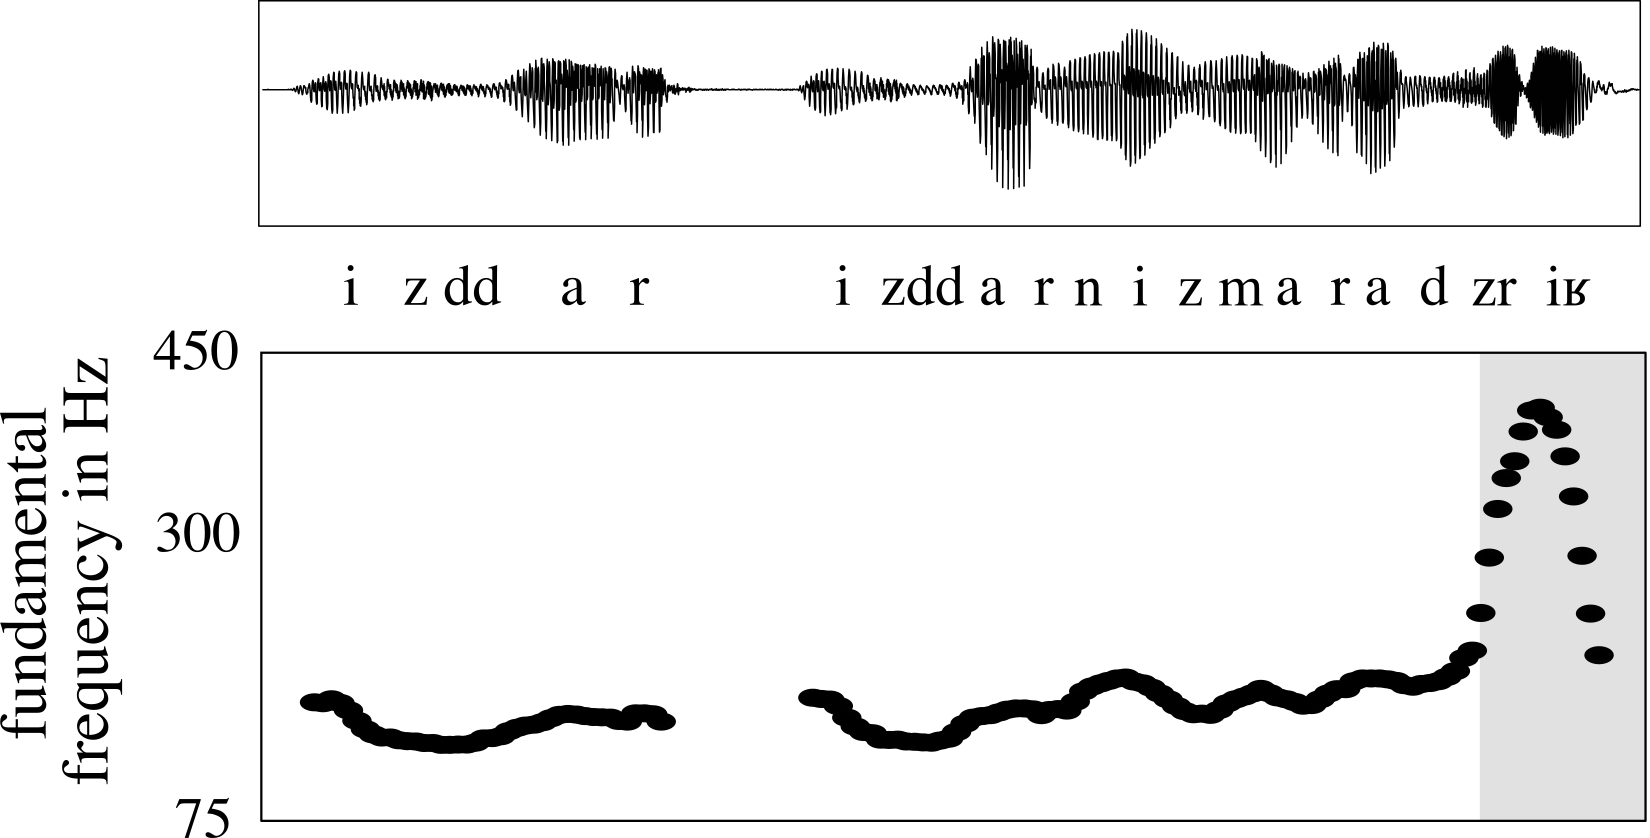
\includegraphics[width=0.8\textwidth]{figures/Figure_5_2_echo.png}
  \caption{Representative waveform and f0 contour of the declarative question /izddar izddar n izm aʁ rad zriʁ/ ‘The bottom… the bottom of the lion is it that I will go?’ Final syllable highlighted in grey.}
   \label{fig:5.2}
   \end{figure}

\subsection{Contrastive focus in Tashlhiyt}
Contrastive focus can be morphosyntactically expressed using either left dislocation or clefting. In both cases, the contrasted or emphasised element appears in clause-initial position preceding the verb (left dislocation, cf. \ref{ex:5:10}). In clefted constructions the clause-initial constituent is additionally marked morphologically (cleft, cf. \ref{ex:5:11}).\is{focus}

\ea\label{ex:5:10}
\gll  ddisk	t-sʁa=t	t-fruχ-t \\
      record \textsc{3f.sg}-bought=it \textsc{f}-child.\textsc{bs-f.sg}\\
\glt ‘A record, the girl bought it.’
\z

\ea\label{ex:5:11}
\gll  ddisk ad t-sʁa t-fruχ-t  \\
      record \textsc{ad} \textsc{3f.sg}-bought \textsc{f}-child.\textsc{bs-f.sg}\\
\glt ‘It is a record that the girl bought.’
\z

Due to the frequent use of morphosyntactic constructions expressing focus, examples of contrastive focus expressed by intonation are only seldom found. In these cases, speakers use a rise-fall to mark contrasted constituents in-situ as illustrated in \figref{fig:5.3}. Here, the speaker contrasts /izddar/ ‘underneath’ with /iggi/ ‘above’ via rise-falls at the end of the respective words. The rise is on the final syllable of each preposition.\is{focus}

This type of contrastive focus can be isolated in elicited speech (cf. \figref{fig:5.4}). The rise-fall is located at the right edge of the focused constituent. Similar to the question tune, pitch suddenly falls after reaching the high target and stays low until the end of the utterance. The entire movement is often restricted to one syllable, here the final syllable of the word (highlighted in grey).\is{focus}

\begin{figure}
  \centering 
   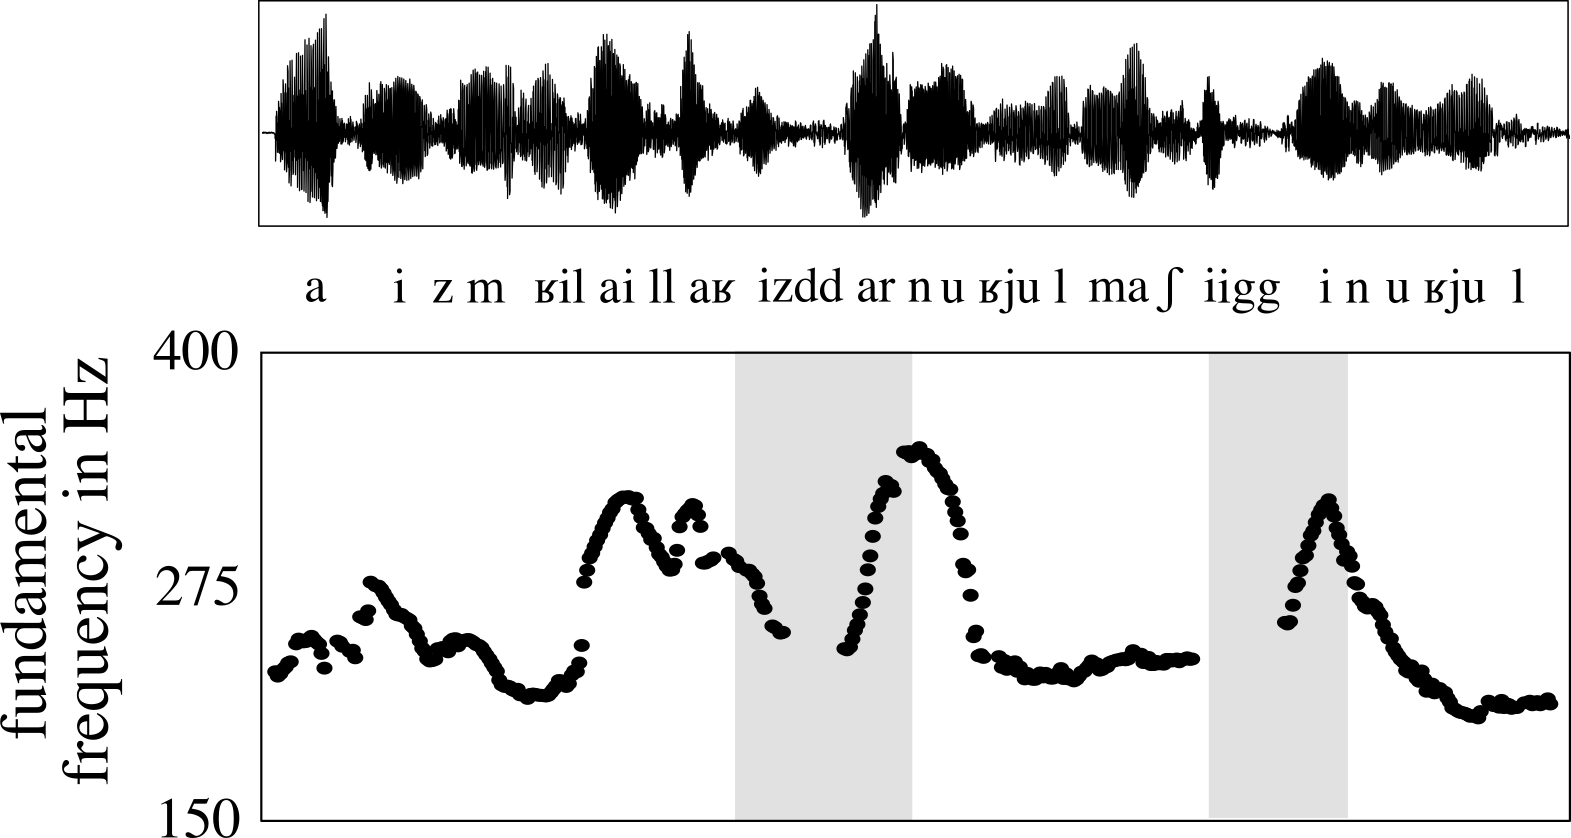
\includegraphics[width=0.8\textwidth]{figures/Figure_5_3_contrast.png}
  \caption{Representative waveform and f0 contour of the statement containing contrasted constituents /a izm ʁila illa ʁ izddar n uʁjul maʃi iggi n uʁjul/ ‘Uh, the lion, now, he is underneath the donkey, not above the donkey’. Contrasted words highlighted in grey.}
   \label{fig:5.3}
   \end{figure}

  \begin{figure}
  \centering 
   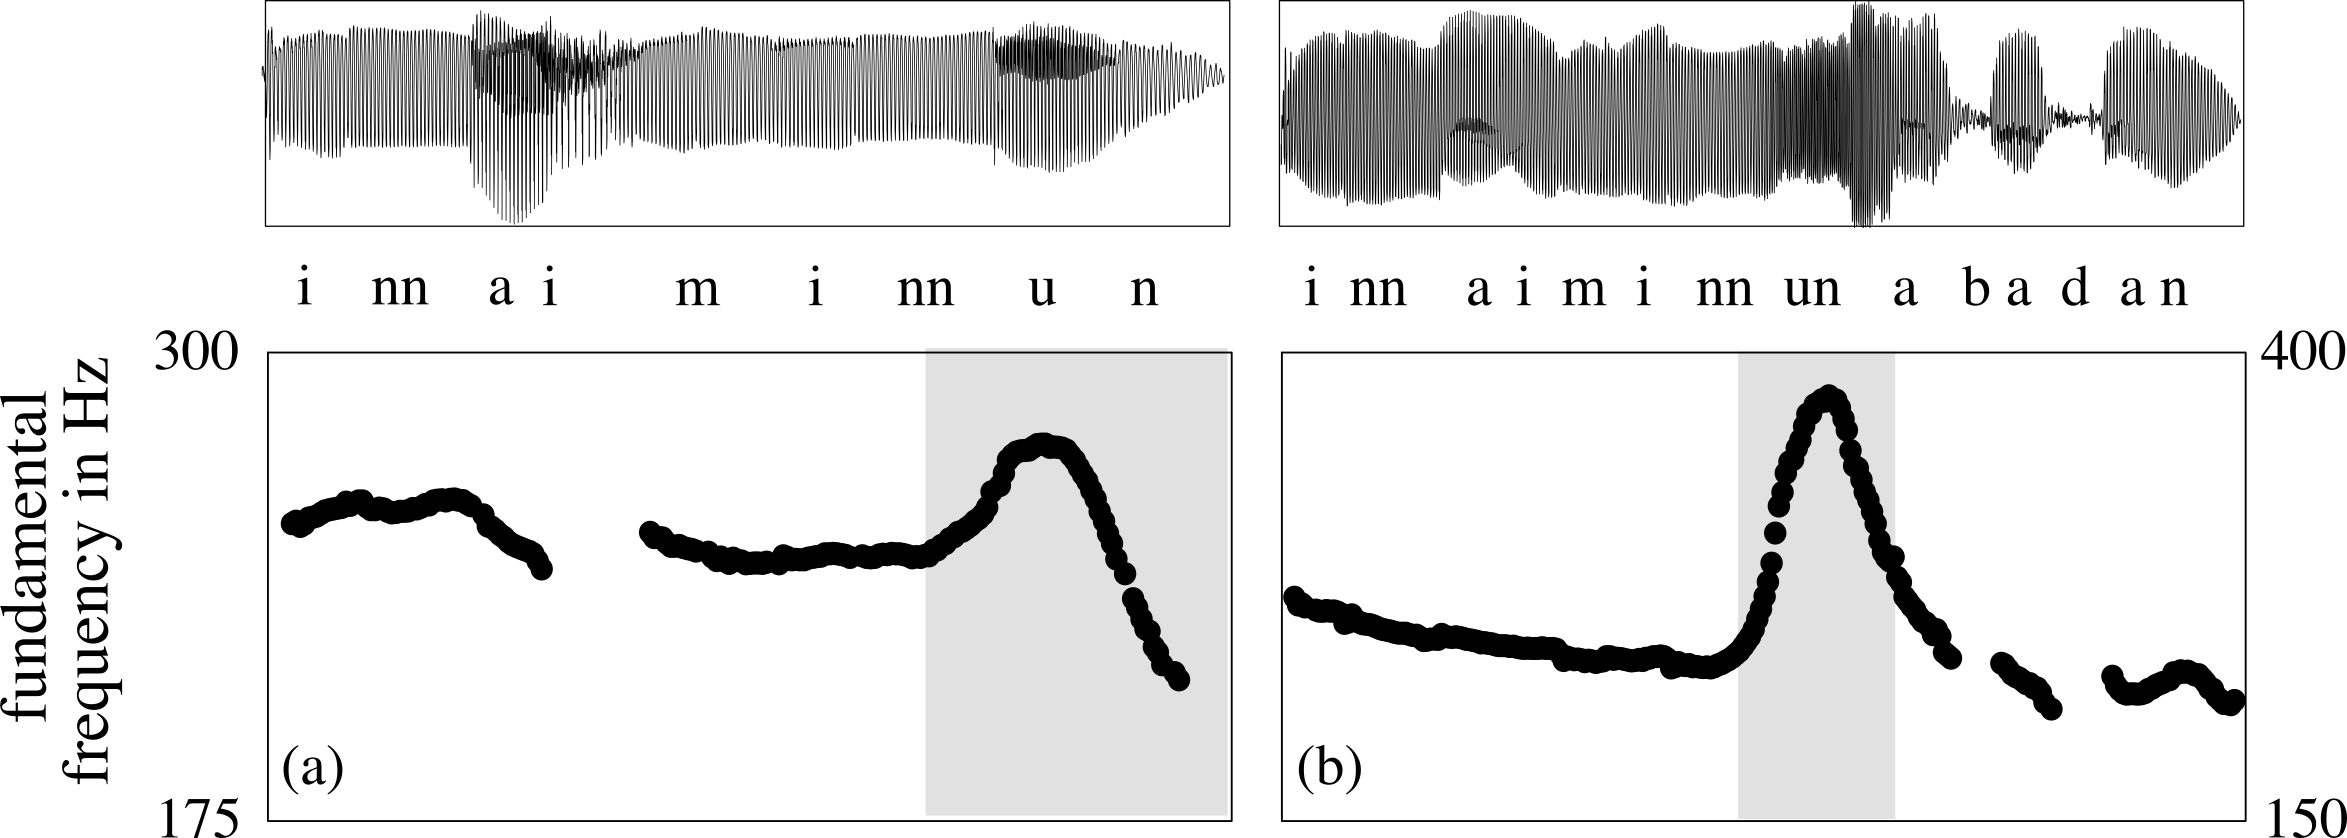
\includegraphics[width=1\textwidth]{figures/Figure_5_4_iminnun.png}
  \caption{Representative waveforms and f0 contours of contrastive statements (a) /inna iminnun/ ‘He said ‘your mouths’.’ and (b) /inna iminnun abadan/ ‘He said ‘your mouths’ always.’. Final syllables of contrasted words highlighted in grey. }
   \label{fig:5.4}
   \end{figure}

\subsection{Intonational differences between flagging questions and marking contrastive focus in Tashlhiyt}
The intonation of questions and contrastive statements are qualitatively similar. Both tunes are characterised by a local rise-fall in pitch. The sentence modalities differ, however, in the position of the rise-fall within the utterance. In contrastive statements, the rise-fall co-occurs with the right edge of the contrasted element. In questions, it co-occurs with the right edge of the phrase. Additionally, the question tune exhibits auditory qualities that distinguish it from the contrastive tune. Comparing the f0 range in questions to the one in statements, it becomes apparent that questions exhibit a higher pitch register, i.e. overall higher f0 values and higher pitch excursion. In fact, speakers frequently change phonation type towards the pitch peak producing a falsetto-like phonation. This is acoustically manifested by strikingly high f0 values of up to 700 Hz and a sudden shift into low vibrational amplitude (\citealt{Laver1994}). The intonation contours of declarative questions and y/n questions resemble each other in terms of both tonal placement and f0 range. \is{pitch scaling}\is{falsetto}

We now set out to evaluate these qualitative observations quantitatively in a controlled reading experiment comparing questions and corresponding contrastive statements, as well as y/n questions and echo questions. 

\section{Production study}\label{sec:5.5}
The objective of the present study is to investigate whether the difference between questions and contrastive statements is reflected in global and local scaling differences and/or in the timing of the rise-fall in pitch. Moreover, echo questions are compared to y/n questions to investigate the potential differences between questions requesting information and questions requesting confirmation. In the following sections, production data from a read speech corpus is analysed. Data has been collected on a field trip in Agadir in November 2013.\footnote{Parts of the analysis presented in this section have been published in \citet{RoettgerGrice2015}.}\is{pitch scaling}

\subsection{Method}
\subsubsection{Participants}
Ten native speakers of Tashlhiyt (five male, five female, mean age = 22 (20-27)) were recorded. All live in Agadir, Morocco, and are fluent in Moroccan Arabic and have basic command of French. All of them had normal or corrected-to-normal vision. None reported on any hearing impairments. Subjects were paid for their participation (cf. Appendix A2.2 for speaker information).

\subsubsection{Speech material}
The present production data is part of a larger corpus of read speech. The read corpus consisted of short mock dialogues containing target words in four different sentence modalities (y/n question, negation, contrastive statement, and echo question) based on the simple sentence: inna \textsc{target} ‘he said \textsc{target}’. Sentences differed with respect to the distance of the target word to the right phrase edge (phrase medial and phrase final). Examples (\ref{ex:5:12}a-d) present the layout of the dialogues with the targets in phrase-final position (no adverb).

\begin{exe}
\ex\label{ex:5:12} \begin{xlist}
                \ex\label{ex:5:12a} is inna \textbf{baba}? \\		
                ‘Did he say ‘father’?’	
                \ex\label{ex:5:12b} ur inna \textbf{baba}. \\ 		
                ‘He did not say ‘father’.’
                \ex\label{ex:5:12c} inna \textbf{dari}.\\ 			
                ‘He said ‘in my house’.’
                \ex\label{ex:5:12d} manik? inna \textbf{dari}? irwas. \\	
                ‘How? He said ‘in my house’? It seems like it.’
\end{xlist}
\end{exe} 

In (\ref{ex:5:12}a) the target word is in a y/n question. In (b) the same target word is in a negative assertion. Because of the preceding negation, a different target word is explicitly corrected in a contrastive statement in (c). Finally, in (d), the proposition in the contrastive statement is called into question in the counter-expectational echo question. In \REF{ex:5:13}, an example dialogue with the target word in phrase-medial position followed by an adverb is given.\footnote{The author is aware of the metalinguistic nature of these context sentences. Exploration of semi-spontaneous and spontaneous speech, however, does not indicate any patterns diverging from the controlled corpus described above. Since target words of different parts of speech were compared, a ‘more natural’ context sentence for the present question was not available.}

\begin{exe}
\ex\label{ex:5:13} \begin{xlist}
                \ex\label{ex:5:13a} is inna \textbf{baba} abadan? \\		
                ‘Did he say ‘father’ then?’	
                \ex\label{ex:5:13b} ur inna \textbf{baba} abadan. \\			
                ‘He did not say ‘father’ then.’
                \ex\label{ex:5:13c} inna \textbf{dari} abadan. \\				
                ‘He said ‘in my house’ then.’
                \ex\label{ex:5:13d} manik? inna \textbf{dari} abadan? irwas. \\	 	
                ‘How? He said ‘in my house’ then? It seems like it.’
\end{xlist}
\end{exe} 

As described above, speakers are expected to produce a rise-fall at the right edge of the phrase in questions (on the target in 12a and \ref{ex:5:12}d, and on the adverb in \ref{ex:5:13}a and \ref{ex:5:13}d). In statements, speakers are expected to produce a rise-fall marking contrastive focus on the target word (phrase final in \ref{ex:5:12}c and phrase medial in \ref{ex:5:13}c). This means that the location of the pitch peak is always either on the target word or on the adverb, in both sentence modalities. The word co-occurring with the pitch peak is henceforth referred to as the ‘tone bearing word’. Productions of the negative assertion in (\ref{ex:5:12}b) and (\ref{ex:5:13}b) are not subject to the present analysis. 

The corpus contained 18 different target words. There were ten fully voiced target words and eight target words containing voiceless segments only. For the present analysis only fully voiced target words are considered (cf. \tabref{tab:5.1}). Each target word appeared in each context at least once. Several items appeared twice. This resulted in 54 fully voiced target words for each participant (total 540). The data with target words containing obstruents only will be subject to discussion in Chapter 6. 

\begin{table}
  \begin{tabular}{ccc}
    \lsptoprule
\textbf{Word}  & \textbf{Translation} \\
    \midrule
ba.ba & ‘my father'\\
da.ri & ‘in my house'\\
di.ma & ‘always'\\
il.di & ‘he pulls'\\
i.min.nun & ‘your mouths'\\
ma.na.gu & ‘when'\\
ʁi.la & ‘now'\\
u.dm & ‘face'\\
\lspbottomrule
  \end{tabular}
  \caption{Target words and translations of production study.}
  \label{tab:5.1}
\end{table} 

\subsubsection{Procedure}
Participants were seated in front of a computer screen and read out orthographically presented material containing the target words as presented in carrier sentences in \REF{ex:5:12} to \REF{ex:5:13} (i.e. in mock dialogues). Participants were asked to enact these dialogues. The materials were presented in a version of the Latin script speakers are used to reading and writing in (see Chapter 3).

Recordings were made in a quiet room at the Ibn Zohr University in Agadir. The production data was recorded using a Marantz PMD 670 solid-state recorder at a sampling rate of 44.1 kHz, and an AKG C420 III head-mounted microphone. Before recordings began, participants were asked to read aloud a word list containing all of the target words to ensure that they were familiar with the words and their meanings. Dialogues were presented in random order. 

\subsubsection{Analyses}
All acoustic data was manually annotated employing the following labelling criteria: segment boundaries (and, in turn, syllable and word boundaries) were identified in the acoustic waveform by means of an oscillogram and a wide-band spectrogram. All segmental boundaries of vowels and consonants were labelled at abrupt changes in the spectra at the time at which the closure was formed or released: this was the case for nasals, laterals (especially in the spectra for the intensity of higher formants), and obstruents (at random noise patterns in the higher frequency regions). All acoustic information was automatically extracted via Praat version 5.4 (\citealt{Praat2015}). 

F0 tracks for all utterances were extracted, manually corrected, and smoothed using the Praat script ‘mausmooth’ (\citealt{Mausmooth2015}). The smoothing algorithm levelled out strong microprosodic effects and enabled the inspection of uninterrupted contours. The smoothed contours were used for automatic extraction of the f0 mean of the word /inna/. Since /inna/ is expected to exhibit a relatively flat f0 over the course of the word in the investigated sentence modalities (cf. \figref{fig:5.4}), the mean f0 of /inna/ (in Hz) is taken as a reference level to operationalise ‘pitch level’. Any tonal movement following /inna/ can be assessed in relation to this reference level. Additionally, minimum and maximum f0 values of the utterance were extracted. The difference between minimum and maximum was calculated in semitones (ST) to operationalise ‘pitch range’. Finally, the timing of the rise-fall was investigated. Due to difficulties in reliably measuring low turning points, it is abstracted away from the actual f0 trajectory and focused on the high turning point for both pragmatic functions. Henceforth the high target is referred to as the pitch peak. Peak timing was calculated as the time lag between the acoustic onset of the final syllable within the word and the f0 maximum in seconds (cf. \ref{ex:5:14}a-c):\is{pitch scaling}\is{tonal alignment}

\begin{exe}
\ex\label{ex:5:14} \begin{xlist}
                \ex\label{ex:5:14a} \textsc{pitch level}: mean f0 of the reference word /inna/.
                \ex\label{ex:5:14b} \textsc{pitch range}: difference between maximum and minimum f0 values in ST.
                \ex\label{ex:5:14c} \textsc{f0 max lag}: lag between the onset of the final syllable of the tone bearing word and the f0 maximum. 
\end{xlist}
\end{exe} 

\subsubsection{Statistics}
Sentences produced with hesitation or unnatural phrasing patterns, mispronunciations of the segmental material, or instances exhibiting list intonation were excluded from the analyses. Moreover, most echo questions from speaker F5 were excluded. She produced echo questions with a monotonous contour. Native speakers who did not participate in the experiment judged these to resemble bored statements and thus inappropriate realisations of the intended context. 

Generally, speakers did well in naturally enacting the dialogues, but they had difficulties with reading aloud. This resulted in an unusually large amount of hesitations and mispronunciations. Overall, acoustic parameters for 471 utterances were submitted to statistical analysis (= 7.8\% data loss) and were analysed with generalised linear mixed models, using R (\citealt{R}), the lme4 package (\citealt{Bates.etal2014}), and the multcomp package (\citealt{Hothorn.etal2008}). Fixed effect specification will be given in the relevant paragraphs below. A term for varying intercepts for speakers and for target words was included. Terms for varying slopes were not included, since the data set is rather small and the factorial design was not balanced (asymmetric exclusion of data points frequently leading to converging issues). Speaker-specific tables will be provided to allow for inspection of consistency across speakers. To determine p-values for the main effects / interactions between factors, a model including the main effect / interaction of interest was compared to the same model with no main effect / no interaction via Likelihood Ratio Tests (LRT). 

\subsection{Results: pitch scaling}
First, we will discuss the scaling differences between sentence modalities. Generally, questions exhibit a higher reference pitch level in /inna/ than statements (cf. \figref{fig:5.5}, \tabref{tab:5.2}). This is true for the comparison between contrastive statements (CS, 189 Hz) and both echo questions (EQ, 235 Hz) and y/n questions (Y/N, 264 Hz).\is{pitch scaling}

  \begin{figure}
  \centering 
   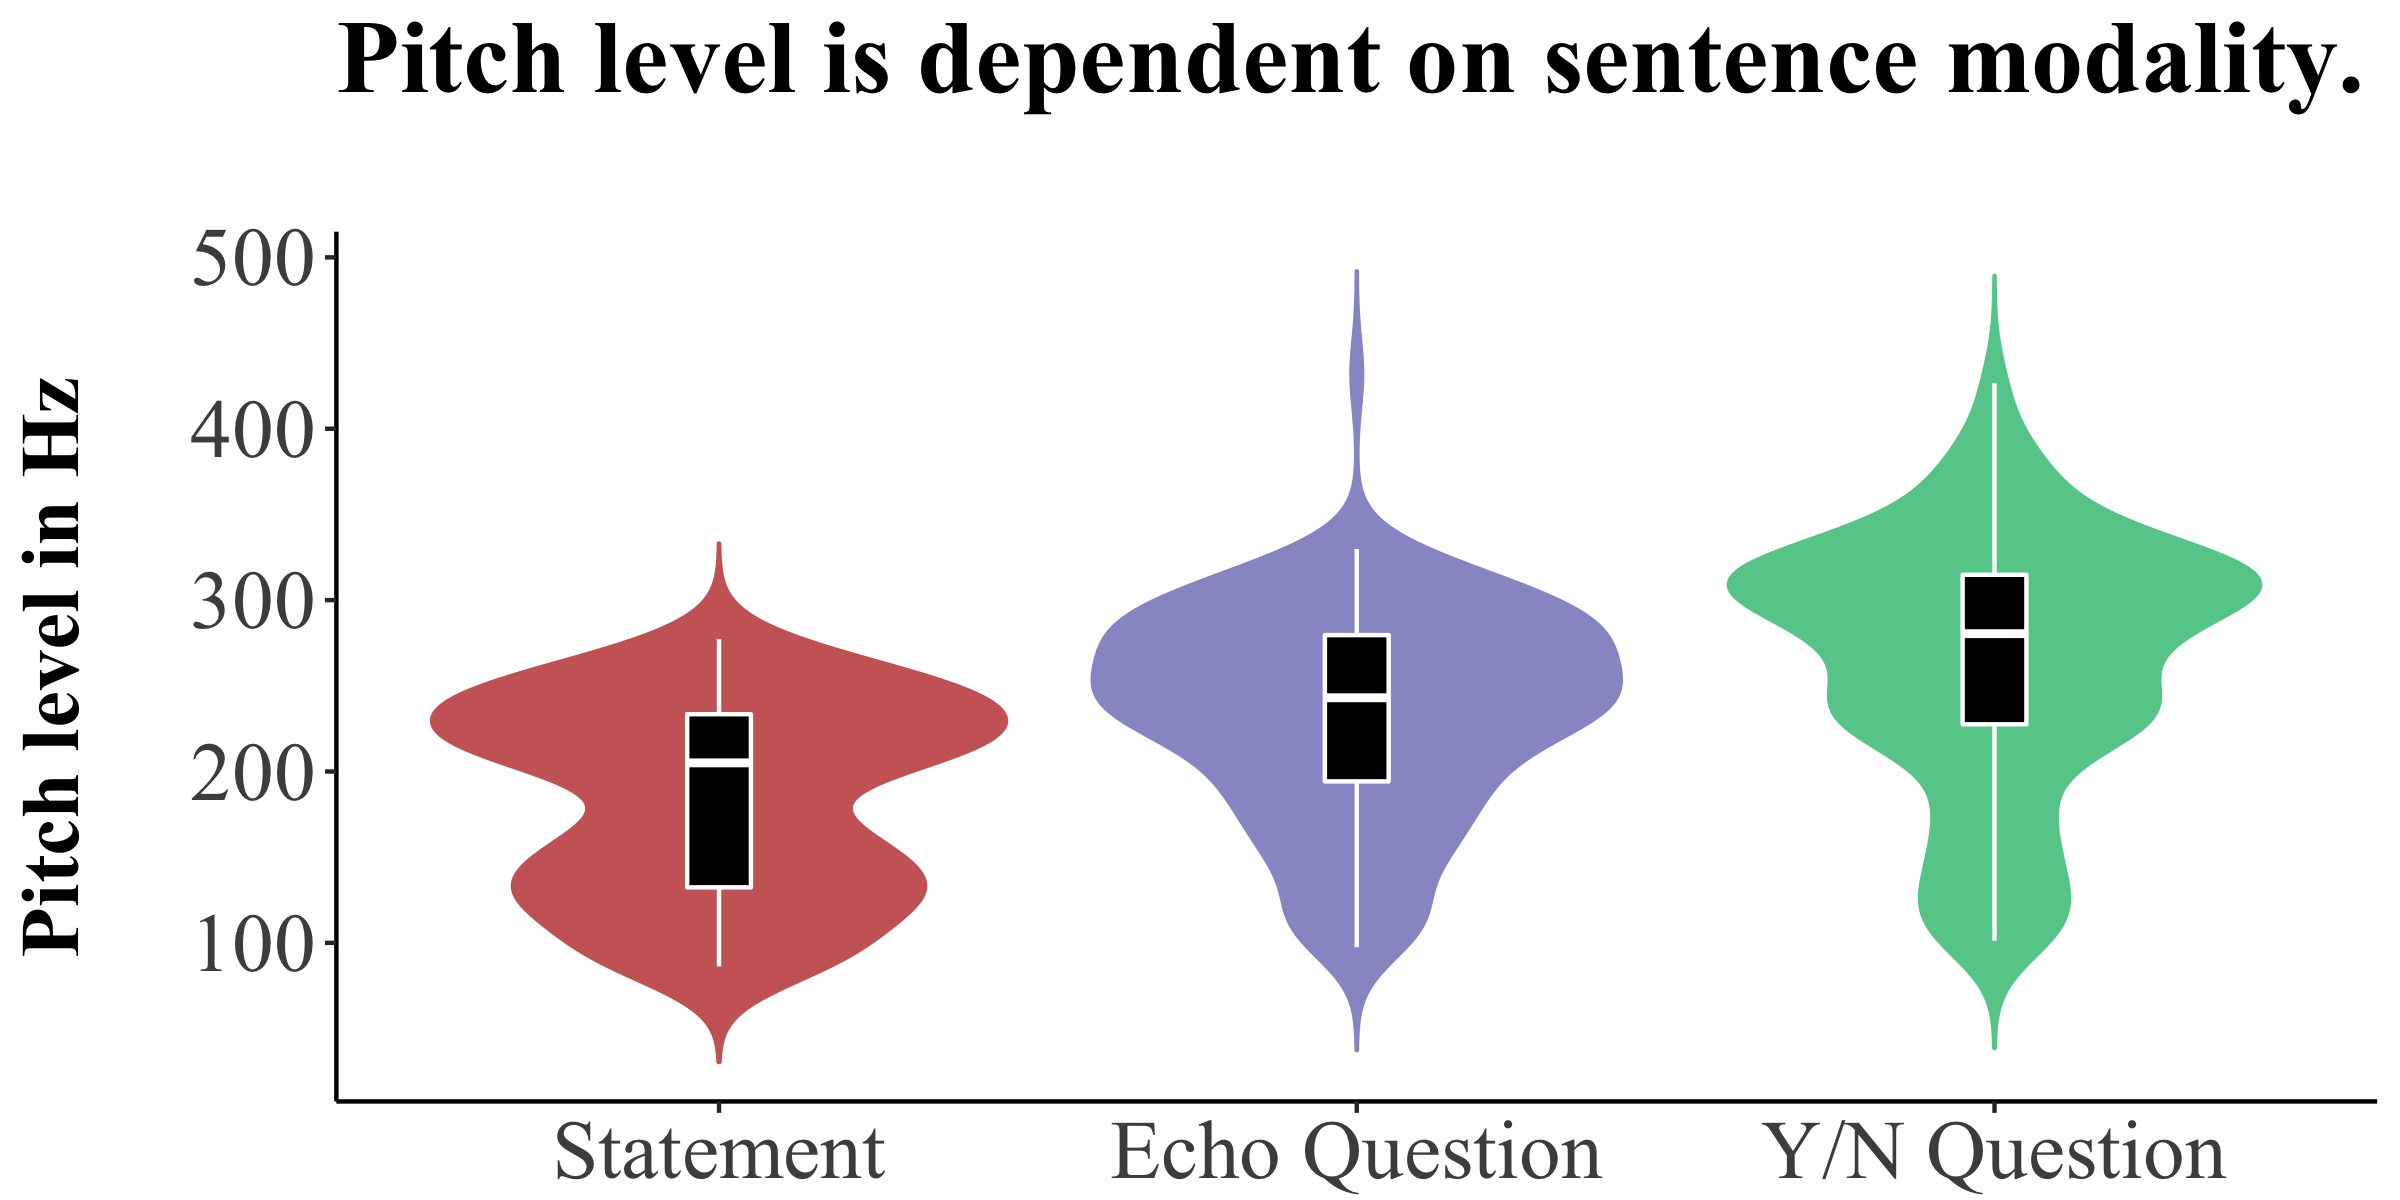
\includegraphics[width=1\textwidth]{figures/Figure_5_5.png}
  \caption{Violin plots of the pitch level values of the reference word /inna/ as a function of sentence modality. Inside each plot, the black boxes indicate the inter-quartile range (IQR), the range between the first and third quartile. The solid horizontal line indicates the median. The whiskers indicate the range, up to 1.5 times the IQR away from the median. The overall shape of the violin plots represent kernel density curves of the raw data distribution.}
   \label{fig:5.5}
   \end{figure}

\begin{table}
  \begin{tabular}{cccc}
    \lsptoprule
\textbf{Speaker} & \textbf{Contrastive Statement} & \textbf{Echo Question} &\textbf{ Y/N Question} \\
    \midrule
F1  & 245 (10)  & 303 (13)  & 317 (20)\\
F2  & 241 (13)  & 298 (40)  & 336 (38)\\
F3  & 217 (5)  & 269 (14)  & 337 (39)\\
F4  & 211 (9)  & 249 (22)  & 280 (25)\\
F5  & 251 (16)  & NA  & 313 (22)\\
M1  & 120 (4)  & 161 (20)  & 168 (19)\\
M2  & 129 (11)  & 194 (12)  & 226 (17)\\
M3  & 152 (11)  & 254 (23)  & 293 (35)\\
M4  & 164 (14)  & 230 (14)  & 237 (16)\\
M5  & 90 (5)  & 110 (8)  & 116(13)\\
\midrule
\textbf{overall} & \textbf{189 (55) } & \textbf{235 (59)}  & \textbf{264 (74)}\\
\lspbottomrule
  \end{tabular}
  \caption{Mean pitch level (and standard deviation, in Hz) of the reference word /inna/ as a function of sentence modality for each speaker individually averaged over words.}
  \label{tab:5.2}
\end{table}

The difference between sentence modalities is consistent across all speakers. Interestingly, echo questions reveal an intermediate status, i.e. they are consistently higher than statements and consistently lower than y/n questions. A linear mixed effects model was performed including sentence modality as a fixed effect. The model estimated the main effect of sentence modality to be significant (χ\textsuperscript{2}(2)=496, p<0.00001). Post-hoc Tukey tests reveal that the difference is in fact significant across all comparisons (statement vs. echo question: β=55.7, SE=2.9, z=19.1, p<0.00001; statement vs. y/n question: β=82.1, SE=2.8, z=29.7, p<0.00001; echo question vs. y/n question: β=26.4, SE=2.8, z=9.5, p<0.00001).\is{pitch scaling}\is{yes-no question}\is{echo question}

We now turn to the pitch range measurements, i.e. the difference between maximum and minimum f0 values within the utterance. Pitch range is numerically rather large with an average of 9 STs across all sentence modalities. In fact, in questions, speakers frequently changed phonation type towards the pitch peak producing a falsetto-like phonation. This is acoustically manifested by very high f0 values of up to 700 Hz and sudden shifts into low vibrational amplitude.\is{pitch scaling}\is{falsetto}

Overall, questions exhibit a greater pitch range than statements. This is true for the comparison between statements (6.8 ST) and both echo questions (10.7 ST) and y/n questions (9.5 ST) (cf. \figref{fig:5.6} and \tabref{tab:5.3}). 

  \begin{figure}
  \centering 
   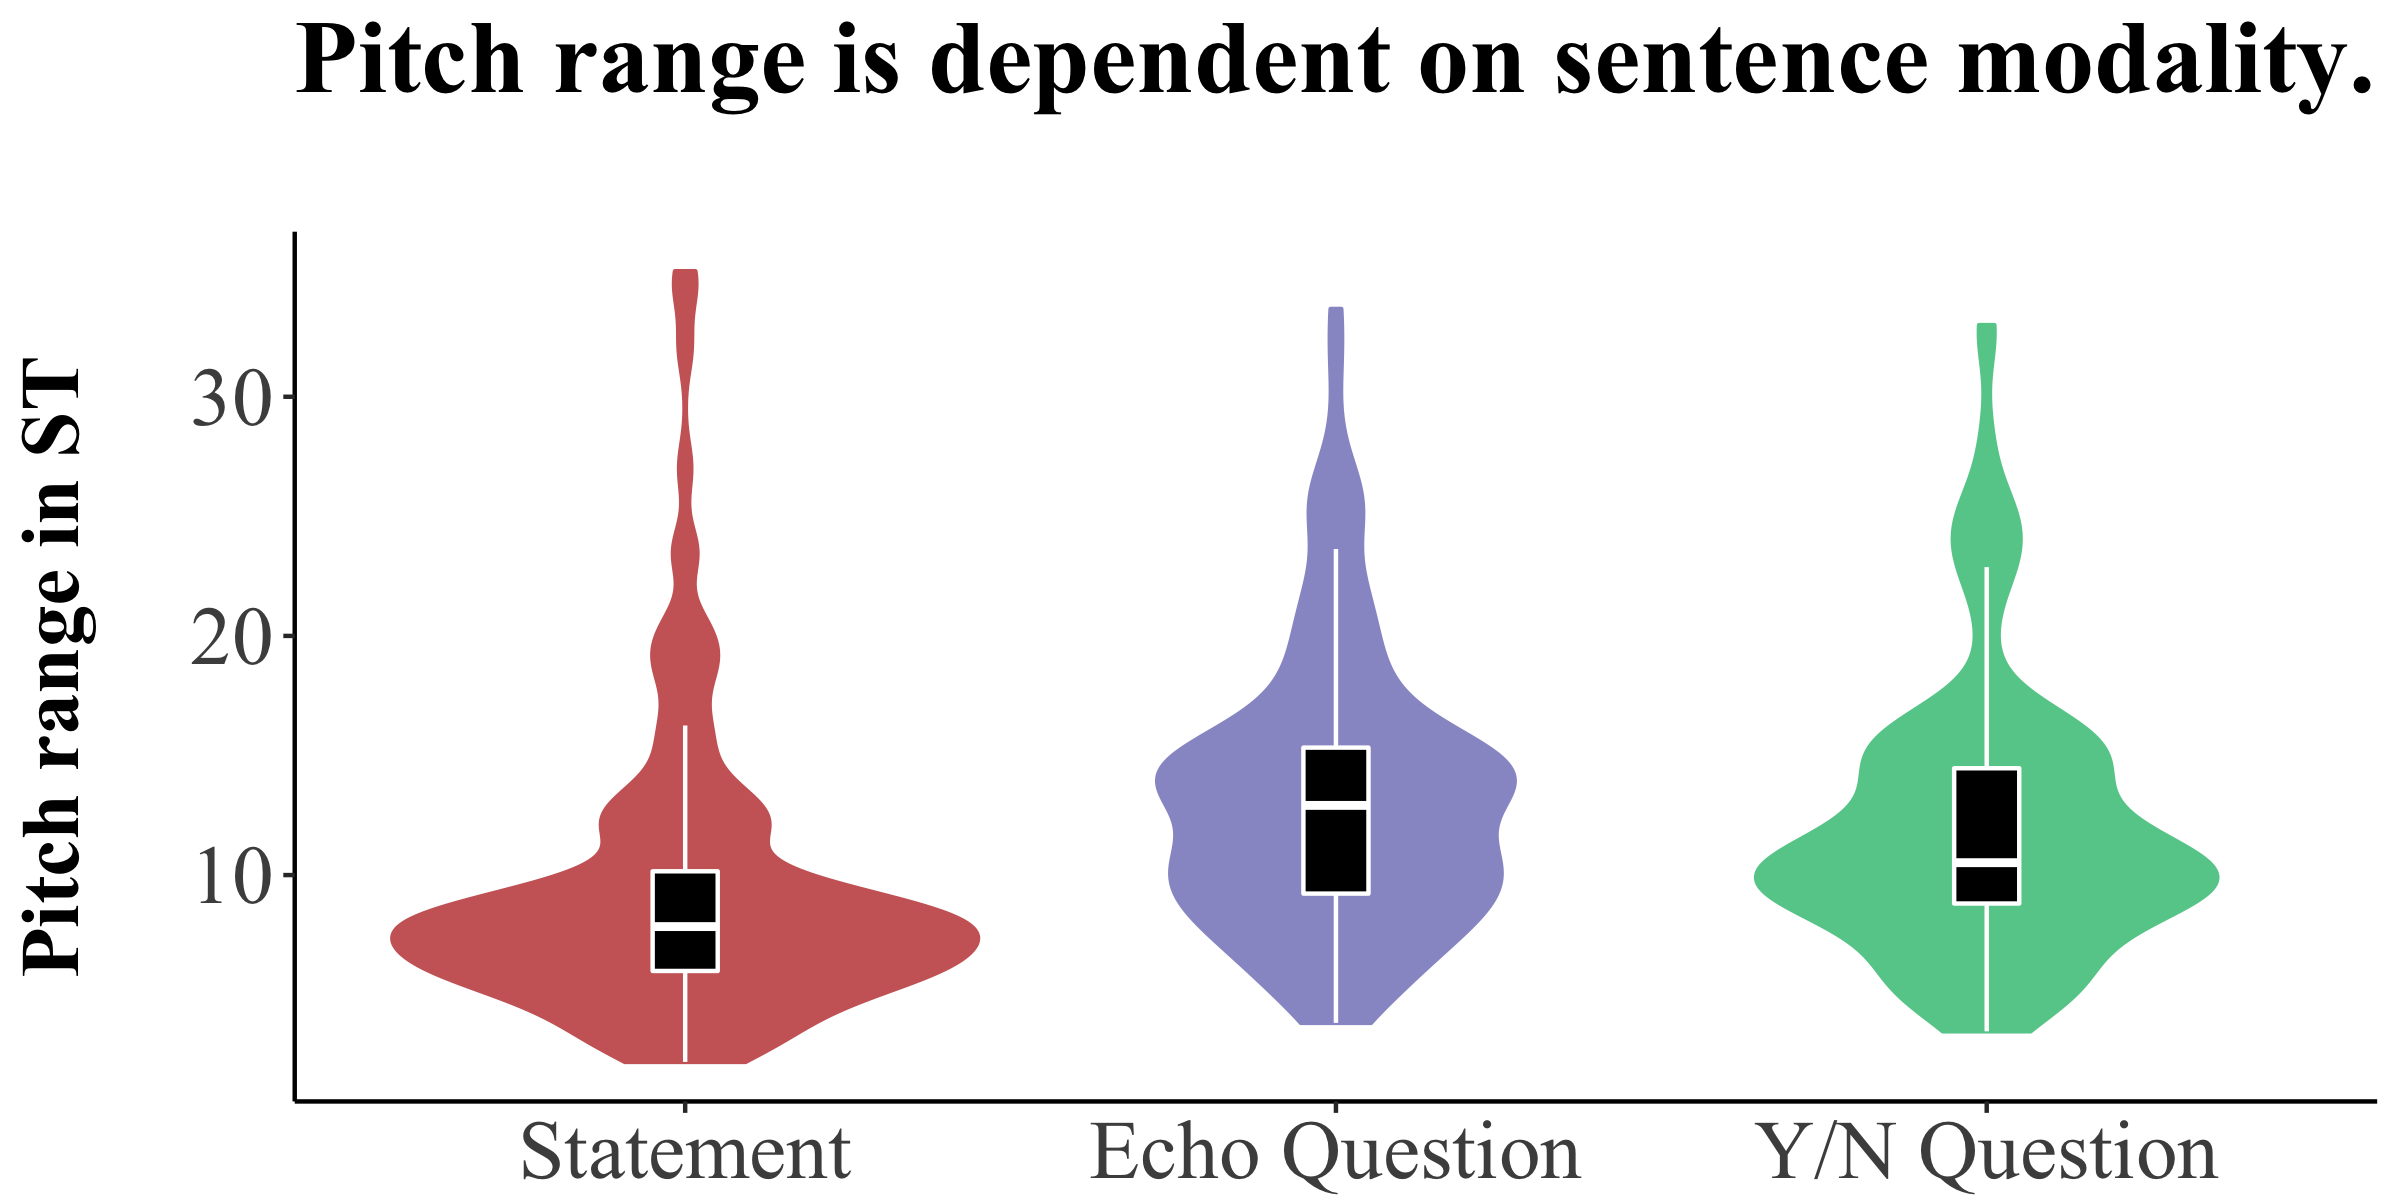
\includegraphics[width=1\textwidth]{figures/Figure_5_6.png}
  \caption{Violin plots of the mean pitch range values as a function of sentence modality. Inside each plot, the black boxes indicate the inter-quartile range (IQR), the range between the first and third quartile. The solid horizontal line indicates the median. The whiskers indicate the range, up to 1.5 times the IQR away from the median. The overall shape of the violin plots represent kernel density curves of the raw data distribution.}
   \label{fig:5.6}
   \end{figure}

\begin{table}
  \begin{tabular}{cccc}
    \lsptoprule
\textbf{Speaker} & \textbf{Contrastive Statement} & \textbf{Echo Question} & \textbf{Y/N Question} \\
    \midrule
F1 & 6.6 (1.7) & 8.4 (1.6) & 7.3 (1.5)\\
F2 & 5.7 (1.6) & 13.3 (2.6) & 13.2 (2.2)\\
F3 & 6.7 (2.7) & 8.2 (2.3) & 10.8 (2.7)\\
F4 & 5.9 (1.2) & 10 (2) & 7.8 (1.3)\\
F5 & 9.1 (3.8) & NA & 10.6 (2)\\
M1 & 3.1 (1.3) & 15.5 (2.5) & 7.6 (3.1)\\
M2 & 6.9 (1.9) & 11.6 (2.1) & 9 (2.8)\\
M3 & 9.8 (1.5) & 14.6 (3.6) & 13.3 (3.6)\\
M4 & 6.5 (3) & 8 (2.3) & 9 (3.2)\\
M5 & 5 (1.4) & 5 (1.8) & 5.8 (1.7)\\
\midrule
\textbf{overall} & \textbf{6.8 (2.8)} & \textbf{10.7 (3.9)} & \textbf{9.5 (3.4)}\\
\lspbottomrule
  \end{tabular}
  \caption{Mean pitch range (and standard deviations, in ST) as a function of sentence modality for each speaker individually averaged over words.}
  \label{tab:5.3}
\end{table}

\newpage 
For some speakers, the distinction between statements and questions is very clear (e.g. F2 and M1), while for other speakers, the distinction is more subtle and characterised by heavy overlap (e.g. F1 and M5). With regard to the distinction between echo questions and y/n questions, there is a large amount of individual variation. Some speakers exhibit a greater pitch range in y/n questions (e.g. F3, M4, M5), while others exhibit a greater pitch range in echo questions (F1, F2, F4, M1, M2, M3) (cf. \tabref{tab:5.3}).\is{pitch scaling}\is{yes-no question}\is{echo question}

A linear mixed effects model was performed including sentence modality as a fixed effect. The model estimated the main effect of sentence modality to be significant (χ\textsuperscript{2}(2)=143.1, p<0.00001). Post-hoc Tukey tests reveal that the difference is in fact significant across all comparisons (statement vs. echo question: β=4.2, SE=0.3 z=12.6, p<0.0001; statement vs. y/n question: β=2.6, SE=0.6, z=4.5, p<0.0001; echo question vs. y/n question: β=1.2, SE=0.3, z=3.9, p=0.0003). Statistically speaking, those speakers that exhibit a greater pitch range in echo questions show a rather strong effect (e.g. speaker M1) which potentially drives the overall mean differences. In light of these inter-individual difference and the fact that the statistical models did not account for varying speaker slopes, generalisations based on the inferential results need to be considered critically here.\is{pitch scaling}\is{yes-no question}\is{echo question}

\subsection{Results: pitch peak timing}
We now turn to the timing of the pitch peak. On average, pitch peaks occurred around 113 ms after the onset of the final syllable of the tone bearing word (utterance final in questions and focused constituent final in contrastive statements). However, the pitch peak is aligned later in y/n questions (144 ms) and echo questions (159 ms) than in statements in which the pitch peak is reached, on average, close to the syllable boundary between the penult and the final syllable (20 ms). A linear mixed effects model was performed including sentence modality as the critical fixed effect. Additionally, the presence of a coda consonant in the final syllable was added in an interaction with sentence modality. This was done because the presence of a voiced coda consonant might enable the pitch peak to be aligned later while still allowing for the full realisation of the subsequent fall (e.g. \citealt{Muecke.etal2009,NiemannMuecke2015}). Here, the presence of a coda consonant actually confounds with the factor sentence modality because there are more cases of tone bearing words with a coda consonant in questions than in statements. Where target words were phrase-medial, the tonal event for questions is always found on the phrase-final adverb /abadan/.\is{tonal alignment}

There is no apparent interaction between the effect of sentence modality and the presence of a coda consonant (χ\textsuperscript{2}(2)=5.49, p=0.064). The model estimates the main effect of sentence modality to be significant (χ\textsuperscript{2}(2)=120.41, p<0.00001). Post-hoc Tukey tests reveal that there is a significant difference between statements and questions, but there is no significant difference between question types (statement vs. echo question: β=0.11, SE=0.01 z=10.9, p<0.0001; statement vs. y/n question: β=0.10, SE=0.01, z=10.3, p<0.0001; echo question vs. y/n question: β=0.01, SE=0.01, z=1.1, p=0.5).\is{tonal alignment}\is{yes-no question}\is{echo question}

It can thus be concluded that the pitch peak in statements is reached earlier in the word than in questions. Echo and y/n questions, on the other hand, appear to have a similar distribution of pitch peak alignment (cf. \figref{fig:5.7}).\is{tonal alignment}\is{yes-no question}\is{echo question}

Looking at the actual distributions of the peak in relation to the onset of the final syllable, it becomes apparent that the averaged values are somewhat misleading (cf. \figref{fig:5.7}). First, the alignment of pitch peaks in statements is more variable than in questions, indicated by the wider spread in the distribution. Moreover, the distribution for statements is not unimodal, but bimodal as indicated by the occurrence of two peaks in the distribution. Looking at questions, there is some indication of bimodality here, too. There is a small bump in the distribution left of the syllable boundary (more prominent in y/n questions). These bimodal distributions reflect the auditory impressions of other researchers (e.g. \citealt{DE1985}, Ridouane p.c.), as well as the impression of the author. Although the pitch peak is most often located on the final syllable, it is possible for speakers to produce the pitch peak on the penult as well. The resulting tonal patterns give rise to discretely different auditory impressions rather than to the impression of a continuously variable position of the tonal event. \is{tonal alignment}

  \begin{figure}
  \centering 
   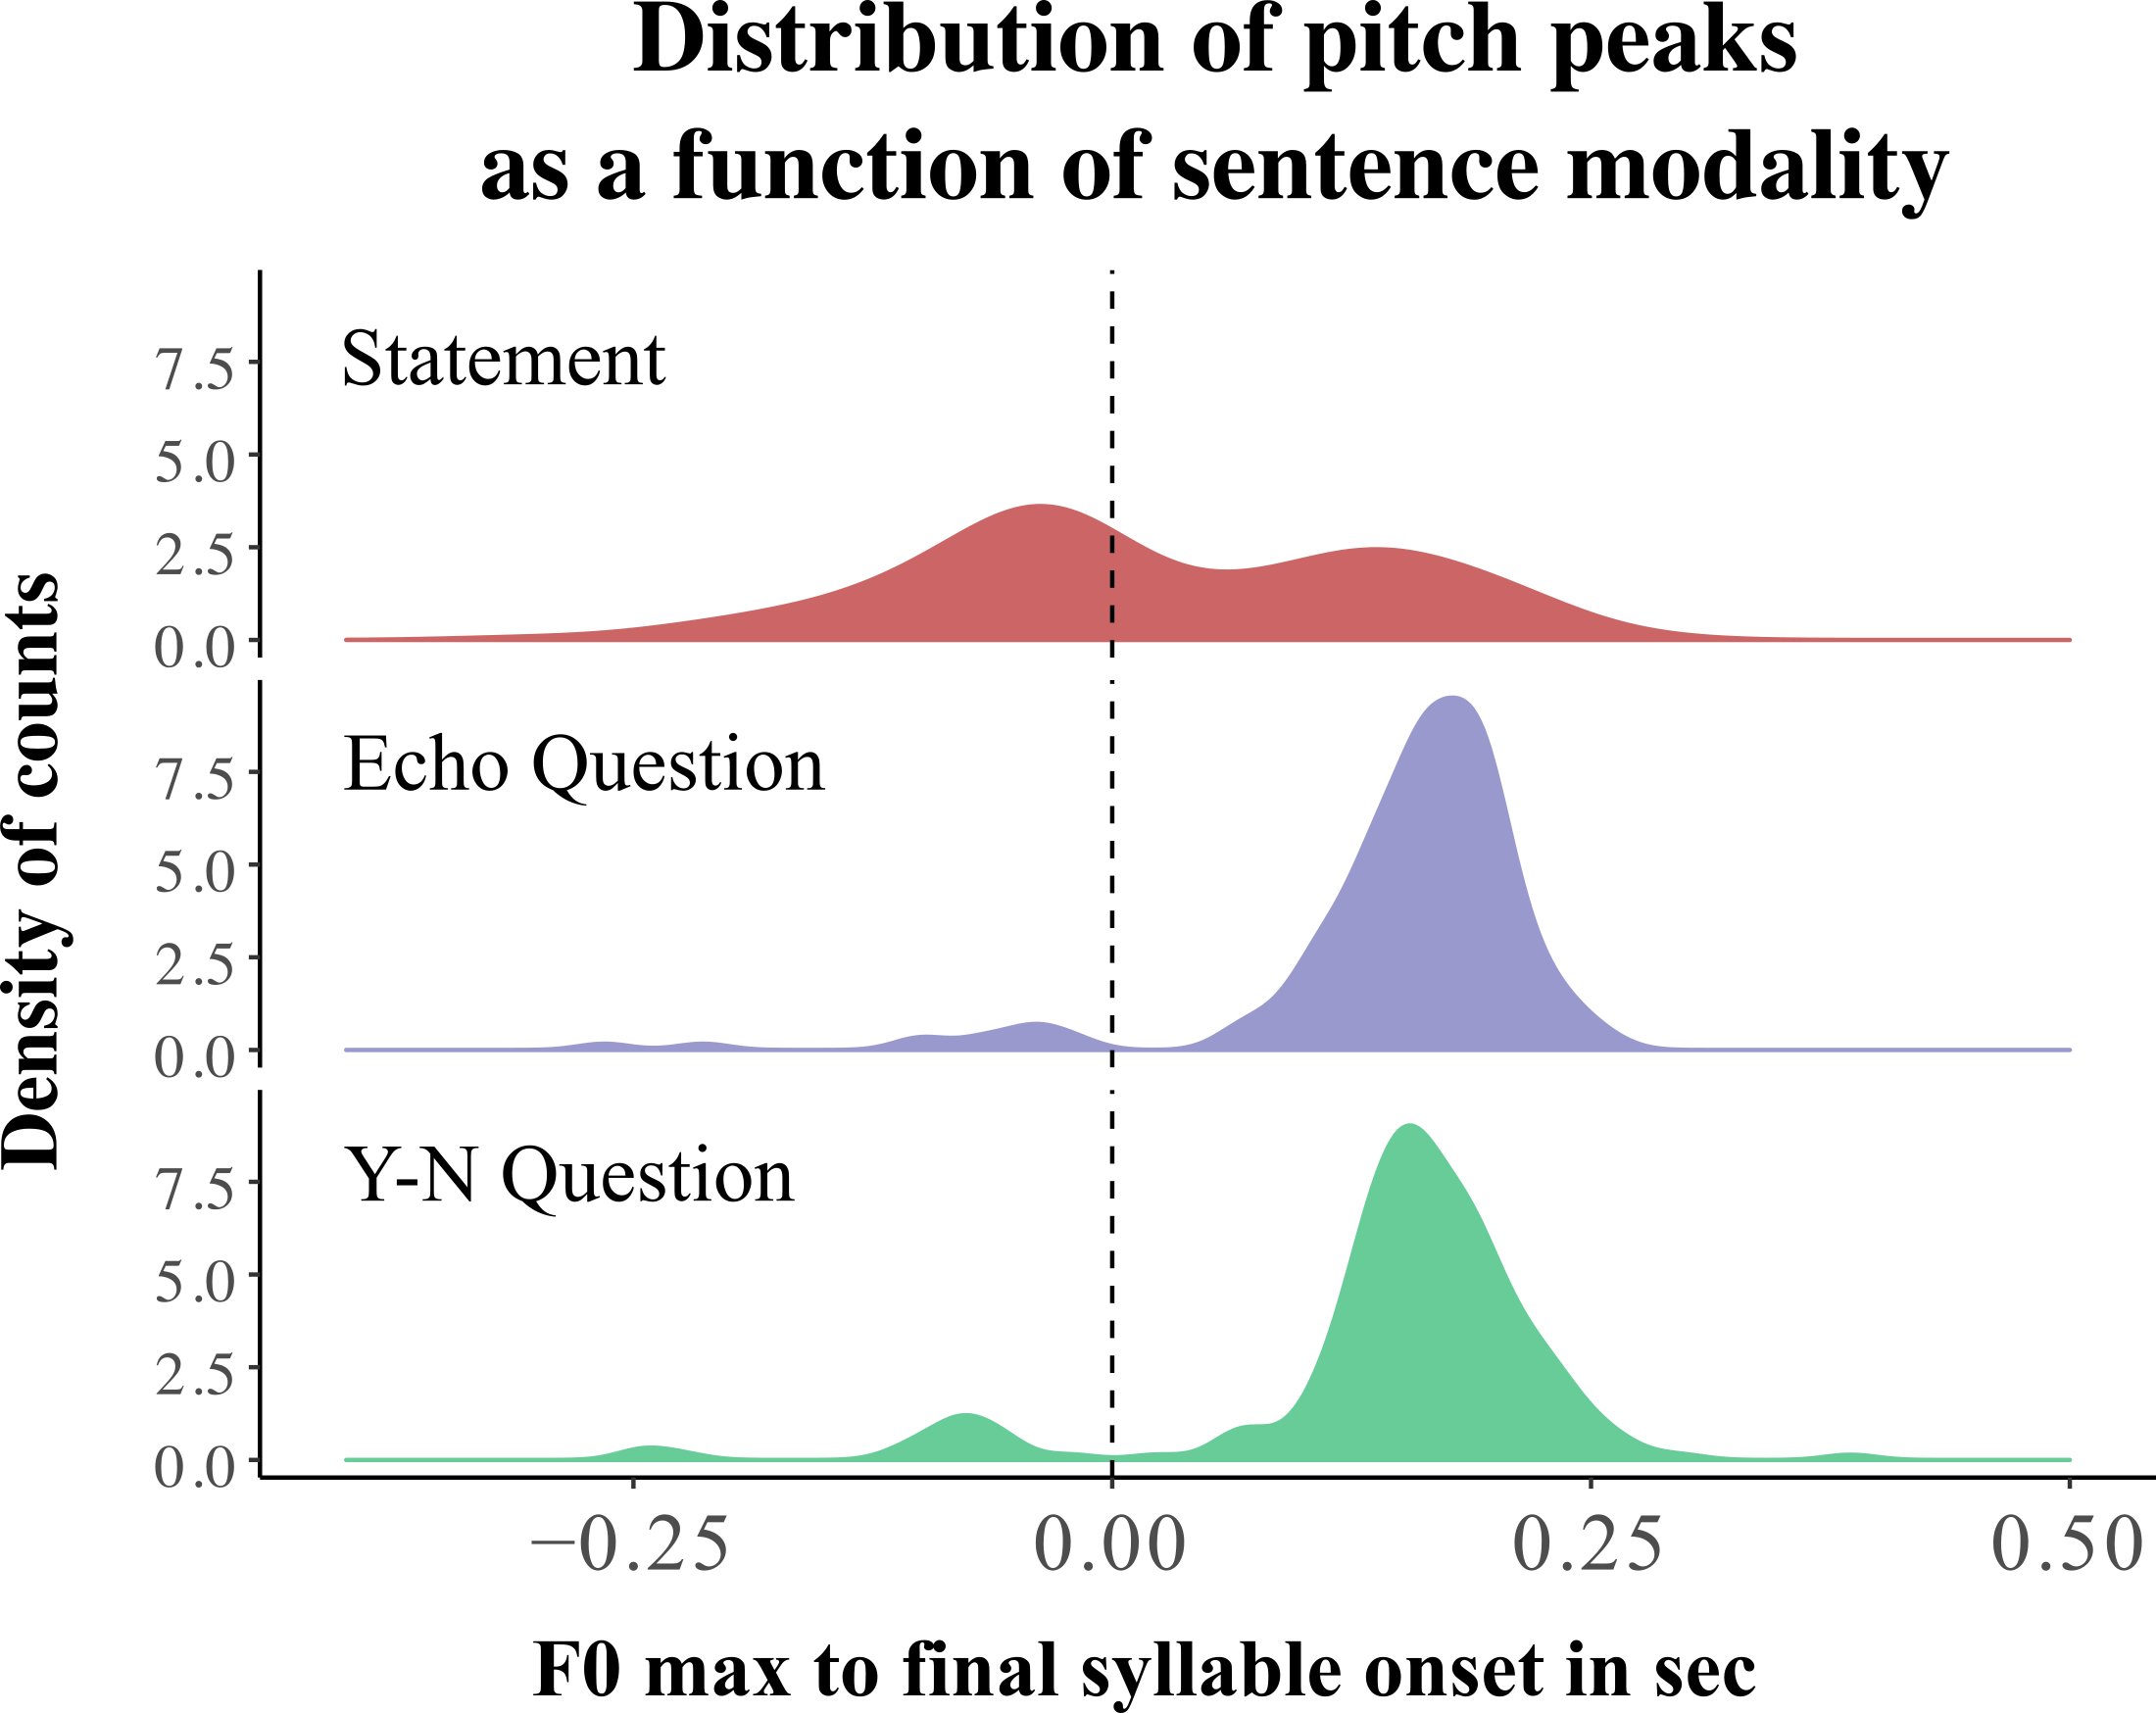
\includegraphics[width=1\textwidth]{figures/Figure_5_7.png}
  \caption{Kernel density curves for pitch peak measurements relative to the onset of the final syllable (at final-to-f0 max = 0) for (a) statements, (b) echo questions, and (c) y/n questions. Positive values indicate that the pitch peak occurs in the final syllable, negative values indicate that the pitch peak occurs in the penult. The dashed line marks the onset of the final syllable.}
   \label{fig:5.7}
   \end{figure}

\tabref{tab:5.4} illustrates the high degree of inter-speaker variability. Generally, there is a strong tendency for individual speakers to produce the pitch peak on the final syllable (most mean values are positive). This trend is stronger for questions than for statements. In fact, some speakers prefer placing the pitch peak on the penult in statements (cf. negative values in M2, M3, and M4). Generally, the pitch peak in statements is found on the penult more frequently than in questions. 

\begin{table}
  \begin{tabular}{cccc}
    \lsptoprule
\textbf{Speaker} & \textbf{Contrastive Statement} & \textbf{Echo Question} & \textbf{Y/N Question} \\
    \midrule
F1 & 17 (127) & 153 (33) & 162 (31)\\
F2 & 36 (111) & 154 (73) & 124 (80)\\
F3 & 53 (118) & 175 (44) & 208 (46)\\
F4 & 30 (105) & 170 (76) & 143 (67)\\
F5 & 23 (157) & NA & 149 (117)\\
M1 & 66 (69) & 126 (54) & 75 (134)\\
M2 & -3 (124) & 147 (22) & 154 (22)\\
M3 & -31 (55) & 147 (71) & 146 (82)\\
M4 & -17 (160) & 177 (67) & 167 (91)\\
M5 & 72 (121) & 111 (133) & 101 (109)\\
\midrule
\textbf{overall} & \textbf{20 (119)} & \textbf{159 (75)} & \textbf{144 (89)}\\
 \lspbottomrule
  \end{tabular}
  \caption{Alignment of mean final-to-f0 max (in ms) with respect to final syllable onset (and standard deviations) as a function of sentence modality for each speaker individually averaged over words.}
  \label{tab:5.4}
\end{table}

This discretely formulated observation is also reflected in more gradual trends in phonetic alignment. Even if only pitch peaks on the final syllable are considered (f0 max lag > 0), the difference between statements and questions holds with statements reaching the pitch peak 129 ms after the onset of the final syllable while echo questions and y/n questions reach the pitch peak later in the syllable (166 and 167 ms, respectively).\is{tonal alignment}

Looking at word-specific distributions, it becomes clear that the mobility of the tonal event appears to be dependent on word-specific properties. \figref{fig:5.8} illustrates the distribution of peak alignment for three representative target words: /i.min.nun/, /ba.ba/, and /u.dm/.

  \begin{figure}
  \centering 
   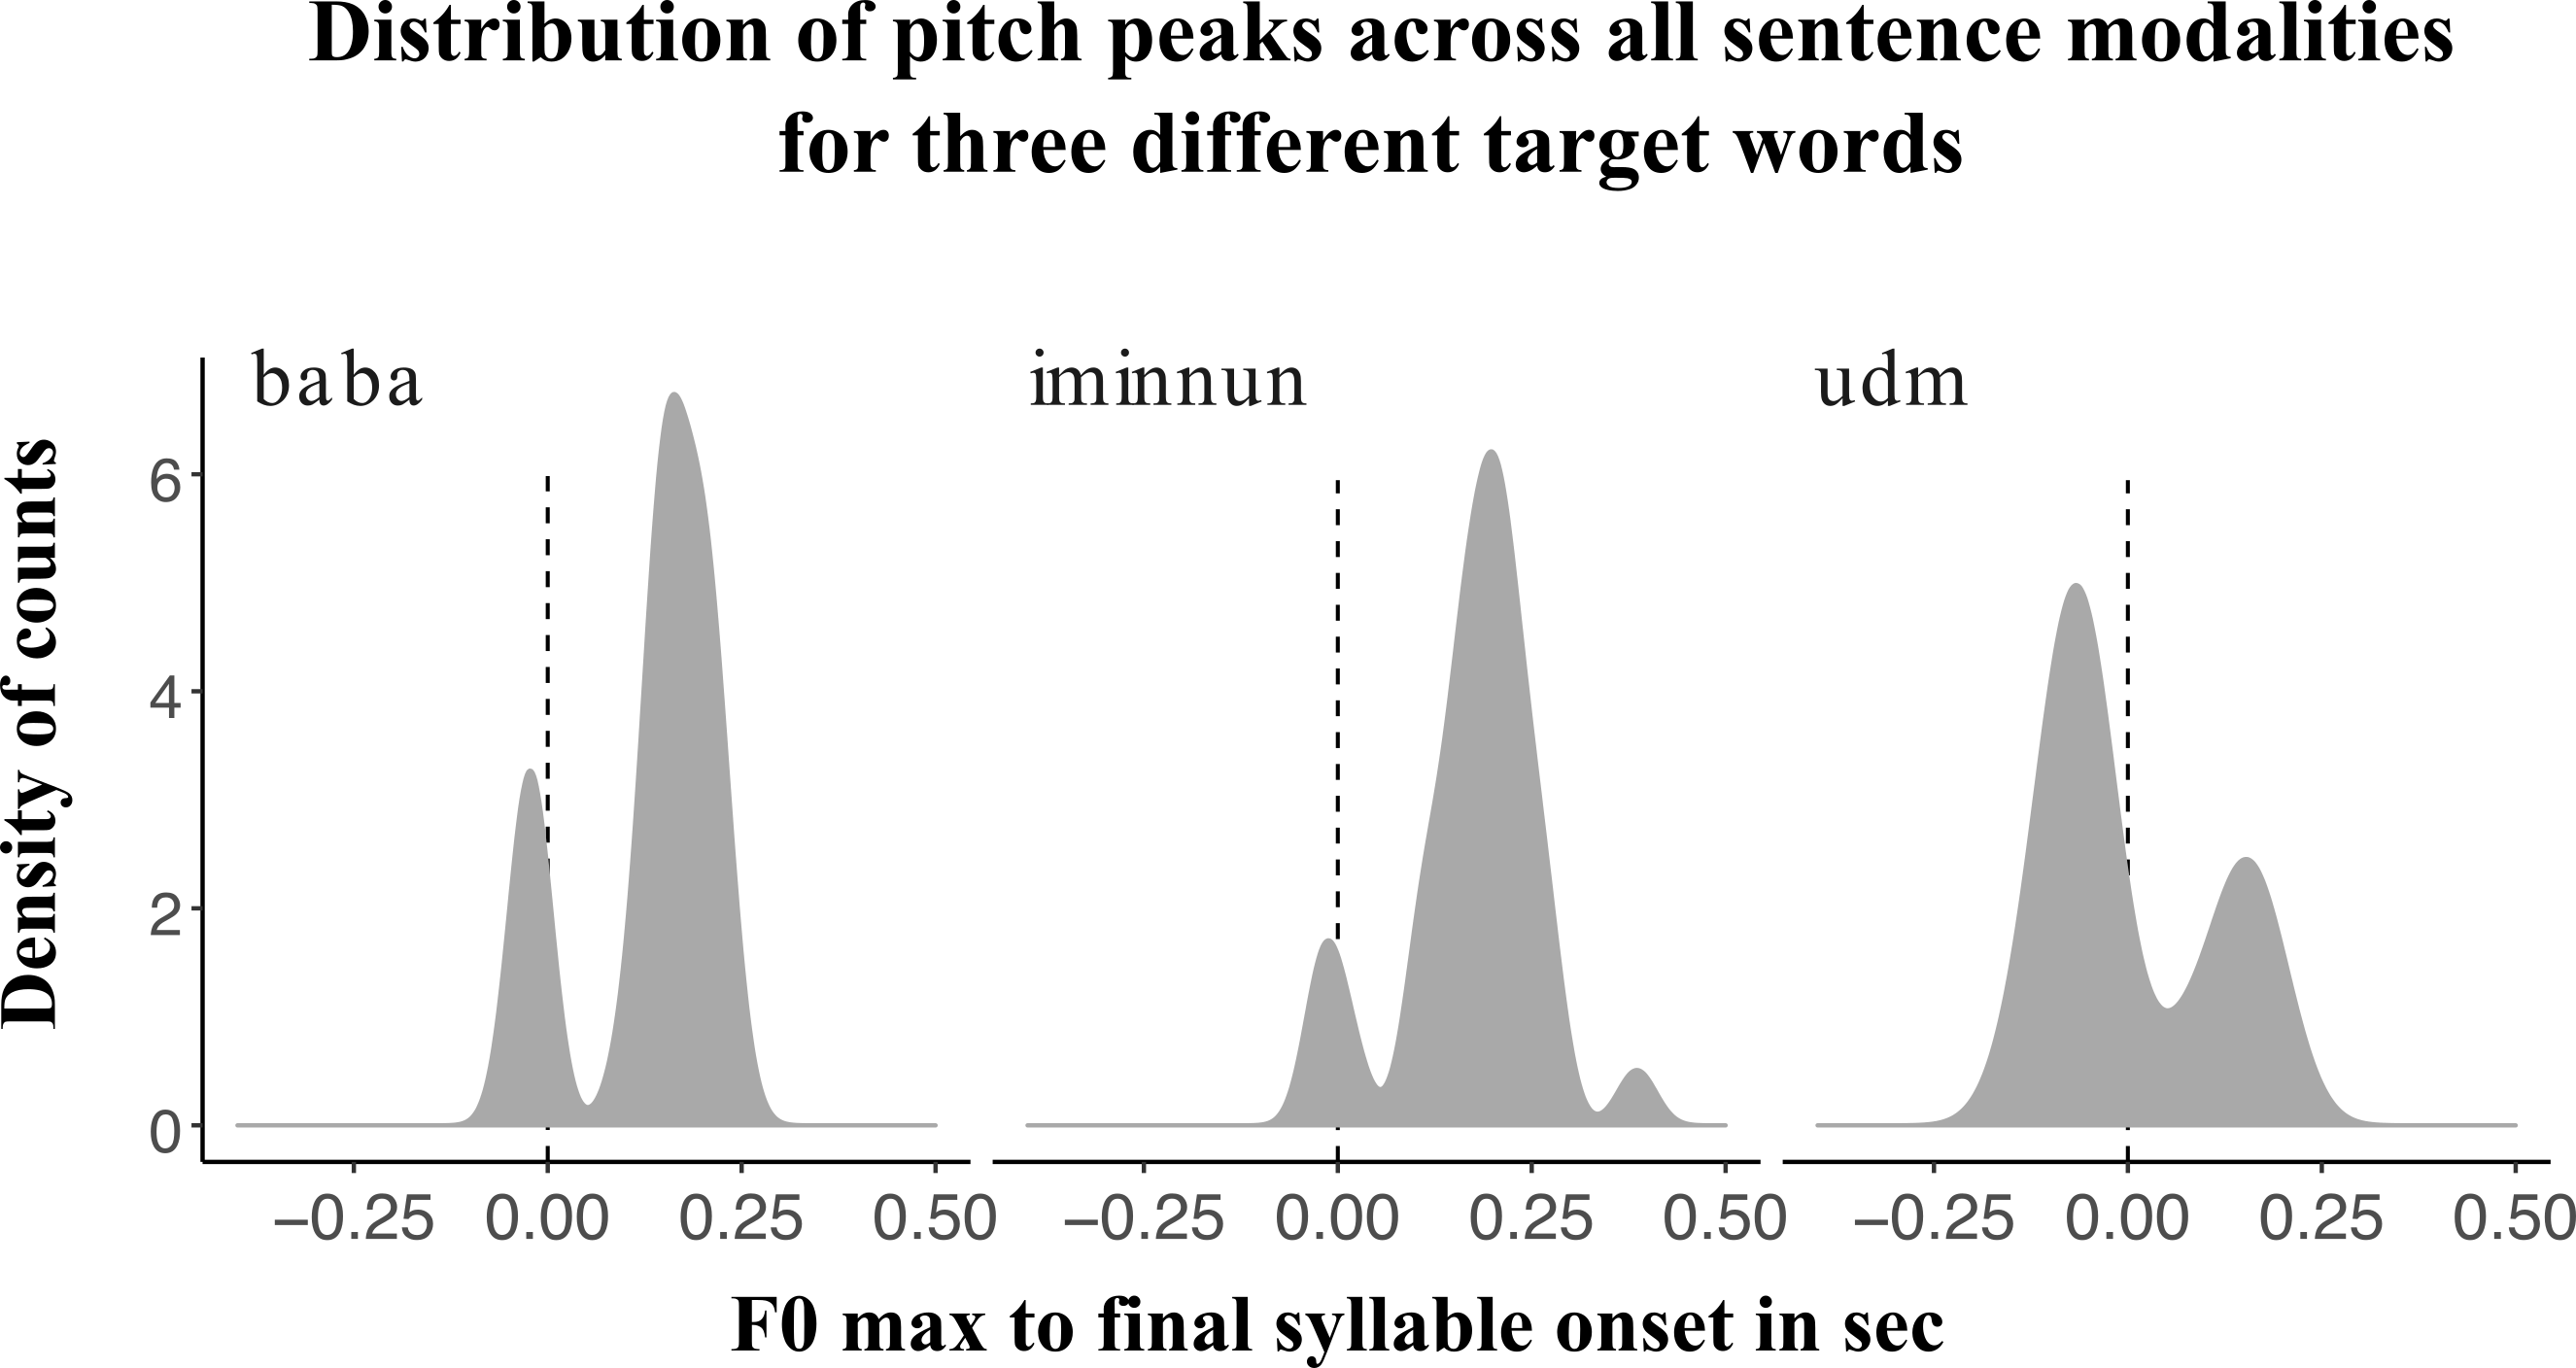
\includegraphics[width=1\textwidth]{figures/Figure_5_8_words.png}
  \caption{Kernel density curve for pitch peak measurements relative to the onset of the final syllable (at final syllable onset to f0 max = 0) for (a) /iminnun/ ‘your mouths’, (b) /baba/ ‘father’, and (c) /udm/ ‘face’. Positive values indicate that the pitch peak occurs in the final syllable, negative values indicate that the pitch peak occurs in the penult. Values are averaged over subjects and sentence modalities. The dashed line marks the onset of the final syllable.}
   \label{fig:5.8}
   \end{figure}

In \figref{fig:5.8}a, there is a subtle bimodality but the majority of peaks appears to be on the final syllable (positive values). In \figref{fig:5.8}b, there is still a strong bias towards the final syllable but also a noticeable amount of peaks occurring on the penult. In \figref{fig:5.8}c, the target /u.dm/ exhibits a strong bimodality with a clear bias towards peaks on the penult. There appears to be something specific about the lexical items that leads speakers to be more likely to produce pitch peaks on the penult or the final syllable. \is{tonal alignment}

\newpage 
In addition to potential lexical effects, in many cases, tonal alignment appears to be prone to some degree of free alternation. \figref{fig:5.9} illustrates examples for the pitch peak on the final syllable and the penult, respectively. In \figref{fig:5.9}a, the penult of /il.di/ is low before f0 suddenly rises towards the peak on the final syllable. In \figref{fig:5.9}b, f0 suddenly drops after reaching its high target on the penult leaving the final syllable low. In most cases, the rise-fall appears to be located exclusively on one syllable.\is{tonal alignment}

  \begin{figure}
  \centering 
   
\includegraphics[width=1\textwidth]{figures/Figure_5_9_ildi.png}
  \caption{Representative waveforms and f0 contours of the contrastive statement /inna ildi abadan/ ‘Did he say ‘he pulls’ always?’ with the pitch peak (a) on the final syllable and (b) on the penult. Syllables co-occurring with the pitch peak are highlighted in grey. Both productions are from the same speaker.}
   \label{fig:5.9}
   \end{figure}

\subsection{Discussion}
To recapitulate the production results, questions in Tashlhiyt are distinguished from corresponding contrastive statements by all three investigated parameters: compared to statements, questions have an overall higher pitch level, a greater pitch range, and the pitch peak is realised later within the word. The alignment pattern can be described in both discrete as well as continuous terms. In questions, the pitch peak is aligned more often with the final syllable than in statements. Statements have many more instances of pitch peaks aligned to the penult than questions. In continuous terms, even if only pitch peaks on the final syllable are considered, questions have later peaks than corresponding statements.\is{pitch scaling}\is{tonal alignment}

In addition to the distinction between statements and questions, echo questions are distinguished from y/n questions. This distinction is mainly manifested in pitch level with echo questions being lower in pitch than y/n questions. Evidence for echo questions having a greater pitch range is weak at best and the two question types exhibit comparable alignment patterns of the pitch peak. \is{pitch scaling}\is{tonal alignment}\is{yes-no question}\is{echo question}

Generally, there is a high degree of variability both across and within speakers with regard to the position of the pitch peak. While some variability can be explained by functional factors like sentence modality, there remains a substantial amount of unexplained variance. A recent study by \citet{Grice.etal2015tash} shed more light on the factors that determine tonal placement in Tashlhiyt. Their results will be reviewed here briefly. 

Grice et al. recorded Tashlhiyt speakers living in Paris. Four native speakers of Tashlhiyt, originally from Morocco but permanently living in Paris, participated in the experiment. Even though the speakers did not live in Morocco anymore, they were frequently in contact with friends and family there. According to the author's impression (and according to Rachid Ridouane, p.c.), their intonational patterns did not diverge from those speakers recorded in Agadir. 

 
Speakers read out short mock dialogues (\ref{ex:5:15}-\ref{ex:5:17}) similar to the corpus described in the production study above (\sectref{sec:5.4.1}). Twenty-eight pairs of disyllabic target words were recorded. Target words varied in the sonority of the syllable nucleus and in the weight of the final syllable.

\begin{exe}
\ex\label{ex:5:15} is inna \textbf{tugl}? \\ 		
‘Did he \textbf{}say ‘she hung’?’
\ex\label{ex:5:16} ur inna \textbf{tugl}. \\		
‘He did not say ‘she hung’.’
\ex\label{ex:5:17} inna \textbf{tmdl}. \\	
‘He said ‘she buried’.’
\end{exe}

In line with the findings presented above, Grice et al. observed that the phrase-final word bears a pitch peak in both y/n questions and contrastive statements. They described the distribution of the pitch peak as a bimodal pattern, with the pitch peak being aligned either with the penult or with the final syllable of the target word. This discrete pattern coincided with the auditory impression of prominence, i.e. the syllable on which the peak occurred sounded louder and longer to the authors. They explicitly state that the position of the pitch peak was unambiguously identifiable when listening to the utterances. In the following, we will focus on the discrete placement patterns of the pitch peak reported by \citet{Grice.etal2015tash}. \is{yes-no question}\is{focus}

In target words with only one sonorant nucleus (i.e. a sonorant consonant, e.g. /r/ in /tr̩.kz̩, tb̩.dr̩/ ‘she danced, she mentioned’), the pitch peak was almost exclusively located on that syllable. When both syllables had a sonorant nucleus (i.e. a sonorant consonant or vowel, e.g. /tiri, tm̩.dl̩/ ‘she wanted, she buried’) there was no clear preference for a peak on the penult or final syllable. Here, the placement of the peak for both statements and questions was highly complex and subject to the influence of a number of interacting factors. Compared to statements, they found a preference for pitch peaks on the final syllable in questions. Orthogonal to that, they identified two independent factors relevant for determining the location of the pitch peak: 

First, the pitch peak was more likely to co-occur with more sonorous syllable nuclei than with less sonorous syllable nuclei. For example, in a word like /tu.gl̩/ ‘she hung’, the vowel, which has a higher sonority than the liquid, was more likely to attract the pitch peak to the penultimate syllable. Conversely, in a word like /tn̩.za/ ‘it was solved’, the final syllable was more likely to attract the pitch peak. The sonority asymmetry was not only relevant for the distinction between vowels and sonorant consonants, but for the distinction between consonants with differing degrees of sonority, e.g. a liquid was preferred over a nasal (e.g. /tm̩.dl̩/ ‘she buried’ vs. /tr̩.km̩/ ‘she rotted’). Overall, the effect of sonority was stronger for vowels than for sonorant consonants, i.e. vowels were stronger attractors for the pitch peak than consonants.

Second, the pitch peak was more likely to co-occur with heavy syllables than with light syllables. In /tu.glt̩/, the pitch peak was more likely to co-occur with the final syllable than in /tu.gl̩/.\is{syllable weight}

The weighting and interaction of these factors was to some degree speaker-specific, although they generally appeared to be additive and systematic throughout the sample (cf. Tables \ref{tab:5.5}--\ref{tab:5.9}). There was a general preference for the pitch peak to occur on the final syllable indicated by the high overall proportional values. Questions were generally more likely than statements to be produced with a final pitch peak, resulting in ceiling effects for several cells. Heavy syllables systematically attracted a final pitch peak more often than corresponding light syllables and more sonorous nuclei attracted a pitch peak more often than less sonorous nuclei. 

The above-identified factors do not explain, however, the entire variance. In many cases, tonal placement was prone to some degree of free alternation. There were numerous cases where the same speaker produced pitch peaks in different locations within the same target word across different repetitions. \figref{fig:5.10} illustrates a minimal quadruplet with statements and y/n questions.

\begin{table}
\centering
\caption{Results of \citet[250f.]{Grice.etal2015tash}: mean proportion (in \%) of pitch peak location on the final syllable in words containing vowels in contrastive statements for each speaker separately. Results are ordered according to the syllable nuclei of the penult and final syllable (V = vowel, S = sonorant consonant) and syllable weight of the final syllable (light or heavy)}
\label{tab:5.5}
\begin{tabular}{cccccc}
\lsptoprule
      & \multicolumn{5}{c}{\textbf{Contrastive Statements}} \\
      & \multicolumn{5}{c}{\textbf{Words Containing Vowels)}} \\
\cmidrule {2-6}
      & F1    & F2    & M1    & M2   &  Overall \\
\midrule
V.S   & 58.3  & 0     & 66.7  & 75   &  51.1    \\
V.V   & 75    & 0     & 100   & 10   &  47.8    \\
S.V   & 100   & 81.8  & 100   & 100  &  95.8    \\
\midrule
light & 61.1  & 29.4  & 79    & 55.6 &  56.9    \\
heavy & 94.4  & 23.5  & 100   & 75   &  73.9    \\
\lspbottomrule
\end{tabular}
\end{table}

\begin{table}
\centering
\caption{Results of \citet[250f.]{Grice.etal2015tash}: mean proportion (in \%) of pitch peak location on the final syllable in words containing consonants only in contrastive statements for each speaker separately. Results are ordered according to the syllable nuclei of the penult and final syllable (L = Liquid, N = Nasal) and syllable weight of the final syllable (light or heavy).}
\label{tab:5.6}
\begin{tabular}{cccccc}
\lsptoprule
      & \multicolumn{5}{c}{\textbf{Contrastive Statements}}\\
      & \multicolumn{5}{c}{\textbf{(Words Containing no Vowels)}} \\
\cmidrule {2-6}
          & F1        & F2        & M1        & M2       & Overall     \\
\midrule
L.N       & 41.7      & 0         & 58.3      & 50       & 37.5        \\
N.N / L.L & 66.7      & 0         & 75        & 100      & 61.7        \\
N.L       & 100       & 41.7      & 100       & 100      & 84.8        \\
\midrule
light     & 55.6      & 5.9       & 64.7      & 83.3     & 52.9        \\
heavy     & 82.4      & 22.2      & 88.9      & 83.3     & 69          \\
\lspbottomrule
\end{tabular}
\end{table}

\begin{table}
\centering
\caption{Results of \citet[250f.]{Grice.etal2015tash}: mean proportion (in \%) of pitch peak location on the final syllable in words containing vowels in y/n questions for each speaker separately. Results are ordered according to the syllable nuclei of the penult and final syllable (V = vowel, S = sonorant consonant) and syllable weight of the final syllable (light or heavy).}
\label{tab:5.7}
\begin{tabular}{cccccc}
\lsptoprule
      & \multicolumn{5}{c}{\textbf{Y/N Questions}} \\ 
      & \multicolumn{5}{c}{\textbf{(Words Containing Vowels)}} \\
\cmidrule {2-6}
          & F1        & F2        & M1        & M2             & Overall     \\
\midrule
V.S   & 76.9 & 63.6 & 50   & 91.7 &  70.8 \\
V.V   & 100  & 100  & 100  & 100  &   100  \\
S.V   & 100  & 100  & 100  & 100  &   100  \\
\midrule
light & 84.2 & 76.5 & 66.7 & 94.4 &   80.6 \\
heavy & 100  & 100  & 100  & 100  &   100  \\
\lspbottomrule
\end{tabular}
\end{table}

\begin{table}
\centering
\caption{Results of \citet[250f.]{Grice.etal2015tash}: mean proportion (in \%) of pitch peak location on the final syllable in words containing consonants only in y/n questions for each speaker separately. Results are ordered according to the syllable nuclei of the penult and final syllable (L = Liquid, N = Nasal) and syllable weight of the final syllable (light or heavy).}
\label{tab:5.8}
\begin{tabular}{cccccc}
\lsptoprule
      & \multicolumn{5}{c}{\textbf{Y/N Questions}} \\ 
      & \multicolumn{5}{c}{\textbf{(Words Containing no Vowels)}} \\
\cmidrule {2-6}
          & F1        & F2        & M1        & M2             & Overall     \\
\midrule
L.N       & 72.7 & 45.5 & 75   & 75   &   67.4 \\
N.N / L.L & 83.3 & 83.3 & 83.3 & 91.7 &   85.4 \\
N.L       & 100  & 100  & 100  & 100  &   100  \\
\midrule
light     & 72.2 & 61.1 & 72.2 & 77.8 &   70.8 \\
heavy     & 100  & 94.1 & 100  & 100  &   98.6 \\
\lspbottomrule
\end{tabular}
\end{table}

  \begin{figure}
  \centering 
   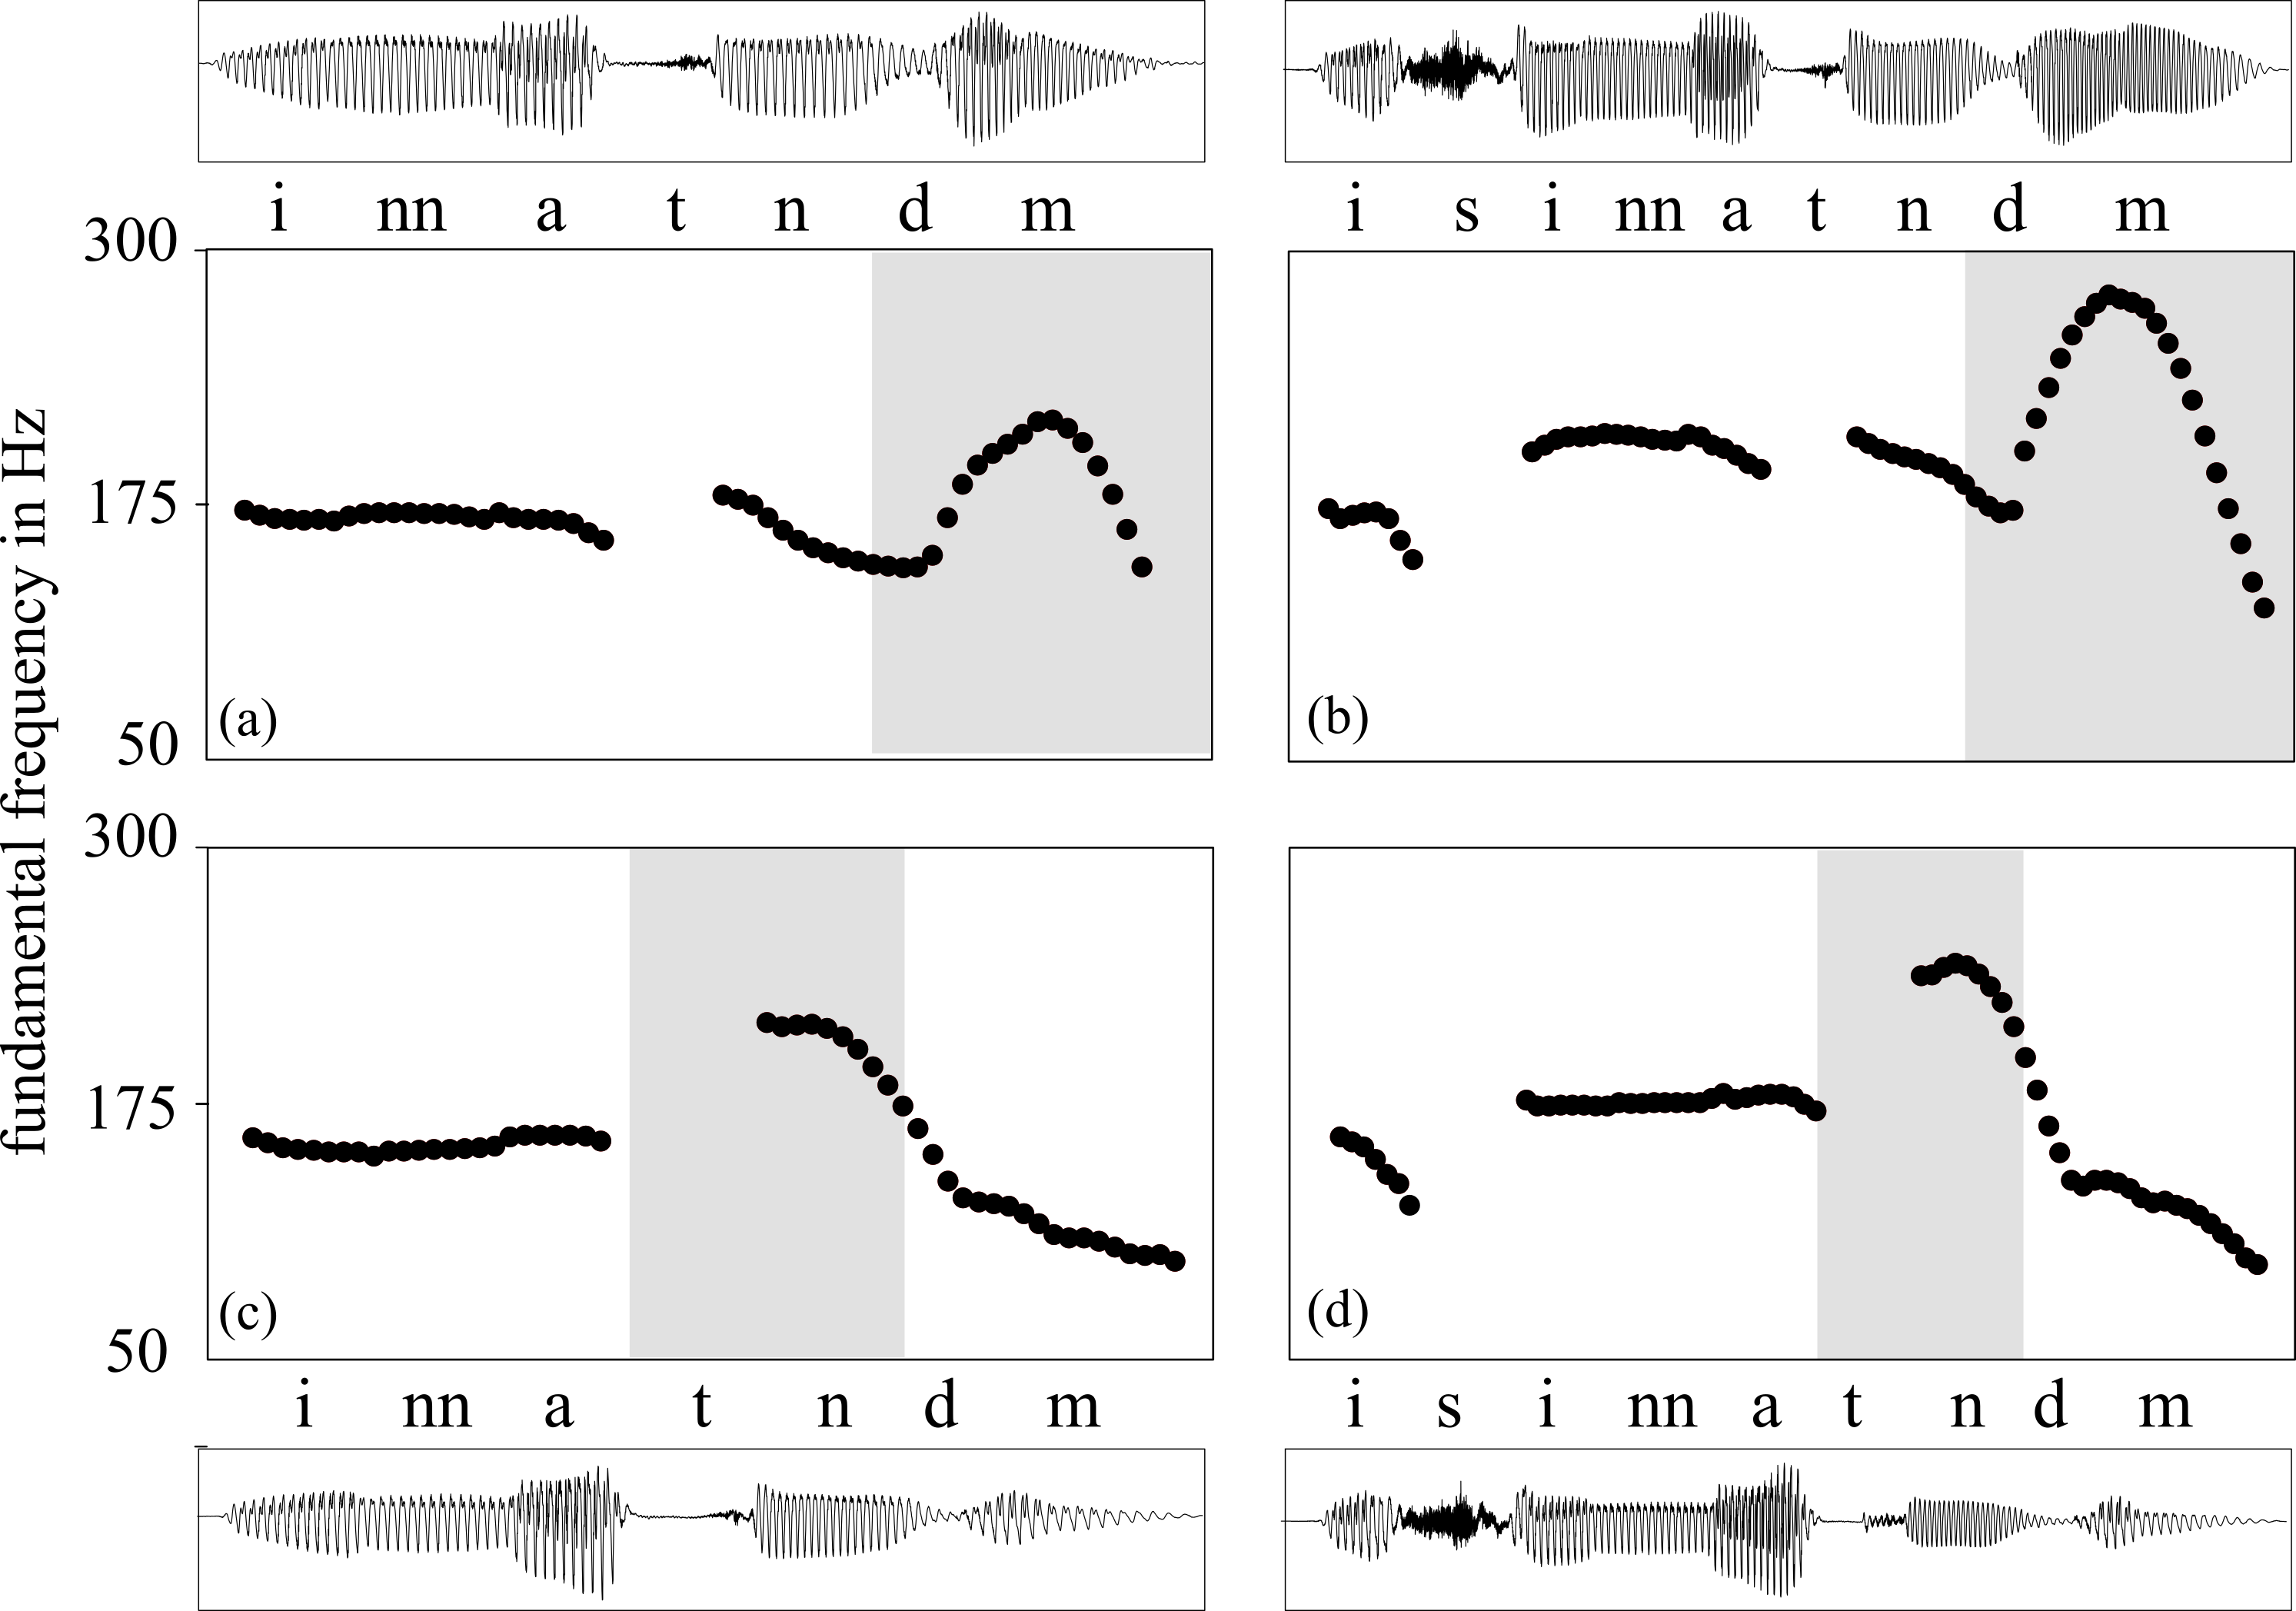
\includegraphics[width=.9\textwidth]{figures/Figure_5_10.png}
  \caption{Representative waveforms and f0 contours of two realisations of the contrastive statement /inna tndm/ ‘he said ‘she regretted’’ (a,c) and the y/n question /is inna tndm/ ‘did he say ‘she regretted’?’ (b,d): the two different realisations for each sentence modality illustrate variation in pitch peak placement. All utterances are from the same male speaker. Tone bearing syllable is highlighted in grey. }
   \label{fig:5.10}
   \end{figure}

  \clearpage  
Grice et al.’s findings put the results of the production study presented in this chapter into perspective. As opposed to Grice et al., there was an even stronger preference for final pitch peaks in the present data set. This might be due to the nature of stimuli employed, i.e. most words had a light final syllable with a vowel in syllable nucleus position. In line with Grice et al., these structures generally attract the pitch peak to the final syllable. Across sentence modalities, the word /u.dm̩/ ‘face’ exhibits an exceptionally large number of pitch peaks on the penult (overall 64\% of all cases across sentence modalities). This may be a reflex of the sonority asymmetry in udm. The vowel in the penult is more sonorous than the nasal in the final syllable and attracts the pitch peak to the penult syllable. The word /i.min.nun/ ‘your mouths’, instead, exhibits mainly final pitch peaks. This is possibly a reflex of the final syllable being heavy. So even though \citet{Grice.etal2015tash} and the present production study had different speaker samples and different speech materials, comparable tonal placement regularities can be observed. \is{syllable weight}

To sum up, Tashlhiyt exhibits a remarkable amount of variability in tonal placement. However, this variability has a particular structure, i.e. it is bimodal. The occurrence of a particular tonal event can only be stated as a probabilistic distribution affected by multiple interacting factors. The question arises if, and if so, how, these probabilistic patterns are used to distinguish sentence modalities perceptually.

\section{Perception study}\label{sec:5.6}
In the preceding section, it has been shown that statements and questions differ in terms of pitch register according to pitch level and pitch range. Moreover, sentence modalities differ with respect to the timing of the tonal event involved. The timing of the pitch peak common to both statements and questions, showed variation in both discrete and continuous terms. The pitch peak co-occurred either with the penult or with the final syllable of the tone bearing word, with more instances of the pitch peak on the final syllable in questions. Moreover, even if only pitch peaks aligned with the final syllable are considered, questions still exhibited a later peak alignment within the syllable. The following perception study investigates whether, and if so, how, Tashlhiyt listeners use these pitch parameters to interpret morphosyntactically ambiguous sentences.\is{pitch scaling}\is{tonal alignment}\is{tone bearing unit}

\subsection{Method}
\subsubsection{Participants}
Nine native speakers of Tashlhiyt (four male, five female, mean age = 21 (20--23)) participated in the experiment. None of them had participated in the previous production experiment. All live in Agadir, Morocco, are fluent in Moroccan Arabic, and have basic command of French. All of them had normal or corrected-to-normal vision. None reported on any hearing impairments (cf. Appendix A2.3 for participant information).

\subsubsection{Speech materials and procedure}
In order to control for pitch register and pitch peak placement, stimuli were resynthesised. As base stimuli, four fully voiced phrases were recorded: /inna baba/, / inna bibi/, / inna dima/, and / inna ʁila/ ‘He said (‘father, turkey, always, now’)’ all produced by a phonetically trained native speaker of Tashlhiyt (Rachid Ridouane). For each phrase, the speaker produced two contours corresponding to two discretely different pitch peak positions resulting in two sets of stimuli: one set contained the pitch peak on the final syllable (F) of the target word and the other set contained the pitch peak on the penult (PU). The speaker was instructed to produce the two sets in the same register. Subsequent inspections of the contours confirmed that this was the case.

Both sets were resynthesised using \uppercase{psola} in Praat version 5.4 (\citealt{Praat2015}). F0 was manipulated resulting in two different pitch register conditions: the low register condition started with a baseline of 130 Hz, the high register condition started 4 semitones higher (  ̴164 Hz). The difference is comparable to values obtained for male speakers in the production study above.

\largerpage[-2]
Generally, f0 was manipulated such that the start of the pitch rise was located at the offset of /inna/ towards two different f0 maximum locations for each set. In the early peak condition, f0 reached its maximum at 1/3 of the way into the vowel (penult vowel in set PU and final vowel in set F). In the late peak condition, f0 reached its maximum at 2/3 of the way into the respective vowel. Note that the alignment differences exceed those typically found in the production study above in order to maximise a potential effect of alignment within the syllable. The maximum f0 value was set to be four semitones higher than the baseline (164 Hz for low register and 206 Hz for high register, respectively). These values are comparable to the typical rise excursions obtained for male speakers in the production study above. After reaching its maximum, f0 fell towards the baseline located at the end of the target word.\footnote{Since the start of the rise and the end of the fall were not identifiable in the production data in a reliable way, the start of the rise and the end of the fall have been fixed to the offset of /inna/ and the end of the utterance accordingly. The potential implications of this methodological choice will be discussed below.}

\largerpage[-2]
These manipulations resulted in 32 stimuli (4 target words * 2 pitch registers (low vs. high) * 2 peak alignments in discrete terms (penult vs. final) * 2 peak alignments in gradual terms (early vs. late)) (cf. \figref{fig:5.11}).\is{pitch scaling}\is{tonal alignment}

  \begin{figure}[t]
  \centering 
   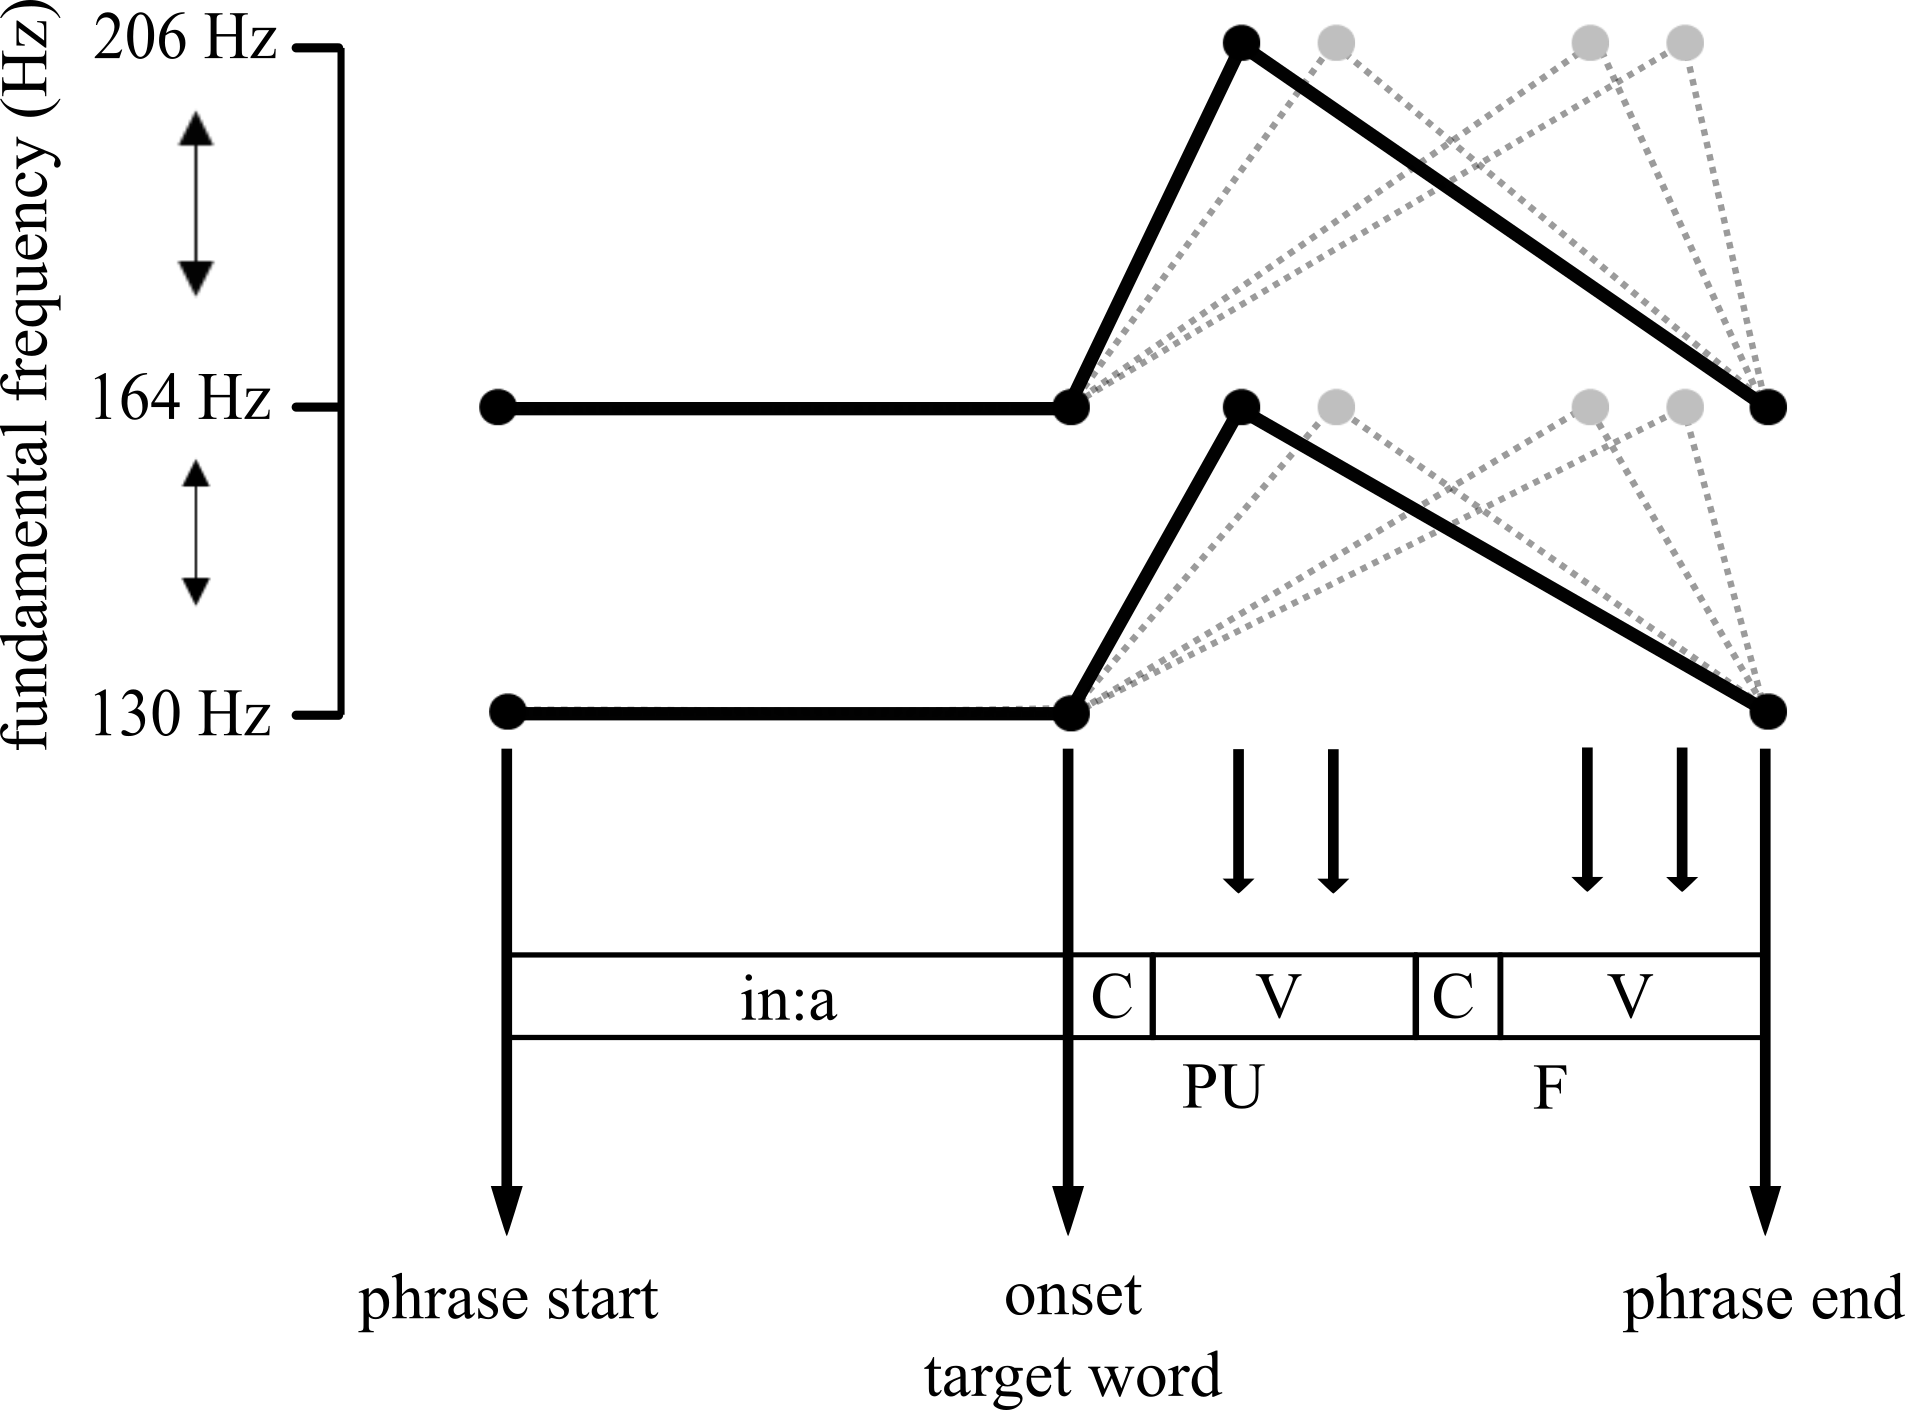
\includegraphics[width=0.75\textwidth]{figures/Figure_5_11_conditions.png}
  \caption{Schematised representation of the manipulation conditions displaying the differences in pitch register, discrete peak alignment (penultimate = PU, final = F), and gradual peak alignment: small arrows indicate early and late alignment within the syllable, respectively.}
   \label{fig:5.11}
   \end{figure}

Participants were seated in front of a computer screen in a quiet room at the Ibn Zohr University in Agadir. They were told that they were going to listen to a robot that speaks Tashlhiyt reasonably well, but has difficulties with producing the difference between statements and questions. Participants were asked to decide whether they would consider the sentences produced as statements or questions by pressing one of two buttons. 

The experiment was run using Superlab (\citealt{Haxby.etal1993}). At the beginning of each trial, a fixation stimulus consisting of a ‘+’ was presented in the centre of the screen for 1500 ms during which participant heard the stimulus. Following this, two sentences appeared on the right and left side of the screen. On one side the statement was displayed in blue (e.g. inna baba ! ), on the other side the question was displayed in red (e.g. inna baba ?). Both were presented in Latin script. The position of the question and the statement was kept constant within participants, but was counterbalanced across participants. Participants had to press the left or right button on the computer keyboard matched with the respective sentence modalities displayed on the screen. After response delivery, a blank screen appeared for 500 ms. 

Each participant started with a training session, in which all combinations of pitch registers and peak alignments (discrete and continuous) were presented once. In subsequent test blocks, each target word in each of the manipulation conditions was repeated five times and presented in randomised order resulting in 160 data points per participant.

\subsubsection{Statistics}
All data was analysed with generalised linear mixed models, using R (\citealt{R}) and the lme4 package (\citealt{Bates.etal2014}). To analyse responses categorically, mixed logistic regression models were used with rating (question or statement) as the dependent measure. Pitch register (low vs. high), discrete peak alignment (PU vs. F), and gradual peak alignment (early vs. late), word, and mean-centred repetition were included as fixed effects. Additionally, a term for random intercepts for participants was included, which quantifies by-participant variability, as well as random slopes for the fixed effects pitch register, discrete peak alignment, and gradual peak alignment for each participant. Models including the main effect / interaction of interest were compared to the same models with no main effect / no interaction via Likelihood Ratio Tests (LRT) to determine p-values.

\subsection{Results and discussion}
Overall, participants rated the stimuli as corresponding to questions in 43\% of the cases indicating a slight bias towards rating the stimuli as statements. This may be due to the declarative syntactic structure of the utterance (no interrogative marker). Regardless of this bias, there was a significant effect of pitch register (χ\textsuperscript{2}(1)=7.5, p=0.006), such that items with a high pitch register were significantly more often rated as questions (58\% vs. 28\%). There was a significant effect of discrete peak alignment (χ\textsuperscript{2}(1)=8.9, p=0.003), as well, such that items with the f0 peak on the final syllable were significantly more often rated as questions than statements (61\% vs. 25\%). Gradual peak alignment did not have a significant effect on ratings. F0 peaks early in a respective syllable were rated as corresponding to questions comparably as often as f0 peaks late in the respective syllable (44\% vs. 41\%) (χ\textsuperscript{2}(1)=1.16, p=0.28, cf. \tabref{tab:5.9}).\is{pitch scaling}\is{tonal alignment}

 \begin{table}[htbp]
  \centering
    \begin{tabular}{cccccc}
\lsptoprule
    \textbf{Register} & \textbf{Discrete Alignment} & \textbf{Gradual Alignment} & \multicolumn{3}{l}{\textbf{Responses}} \\
    \midrule
    \multirow{4}[8]{*}{Low} & \multirow{2}[4]{*}{PU} & early & 0.16 & \multirow{2}[4]{*}{0.15} & \multirow{4}[8]{*}{0.28} \\
\cmidrule{3-4}          &       & late  & 0.14  &       &  \\
\cmidrule{2-5}          & \multirow{2}[4]{*}{F} & early & 0.46  & \multirow{2}[4]{*}{0.40} &  \\
\cmidrule{3-4}          &       & late  & 0.33  &       &  \\
    \midrule
    \multirow{4}[8]{*}{High} & \multirow{2}[4]{*}{PU} & early & 0.31  & \multirow{2}[4]{*}{0.36} & \multirow{4}[8]{*}{0.58} \\
\cmidrule{3-4}          &       & late  & 0.41  &       &  \\
\cmidrule{2-5}          & \multirow{2}[4]{*}{F} & early & 0.82  & \multirow{2}[4]{*}{0.79} &  \\
\cmidrule{3-4}          &       & late  & 0.77  &       &  \\
    \lspbottomrule
    \end{tabular}%
\caption{Mean proportions of question ratings as a function of pitch register (low vs. high) and peak alignment (discrete and gradual).}
  \label{tab:5.9}%
\end{table}% 

\figref{fig:5.12} illustrates the overall results (left panel) and the listener-specific results (right panels) for pitch register and discrete peak alignment. As can be seen, the overall effects of register and discrete alignment appear to be additive, with a final pitch peak in a high register being the preferred question type, and a penultimate pitch peak in a low register being the least preferred question type.

  \begin{figure}
  \centering 
   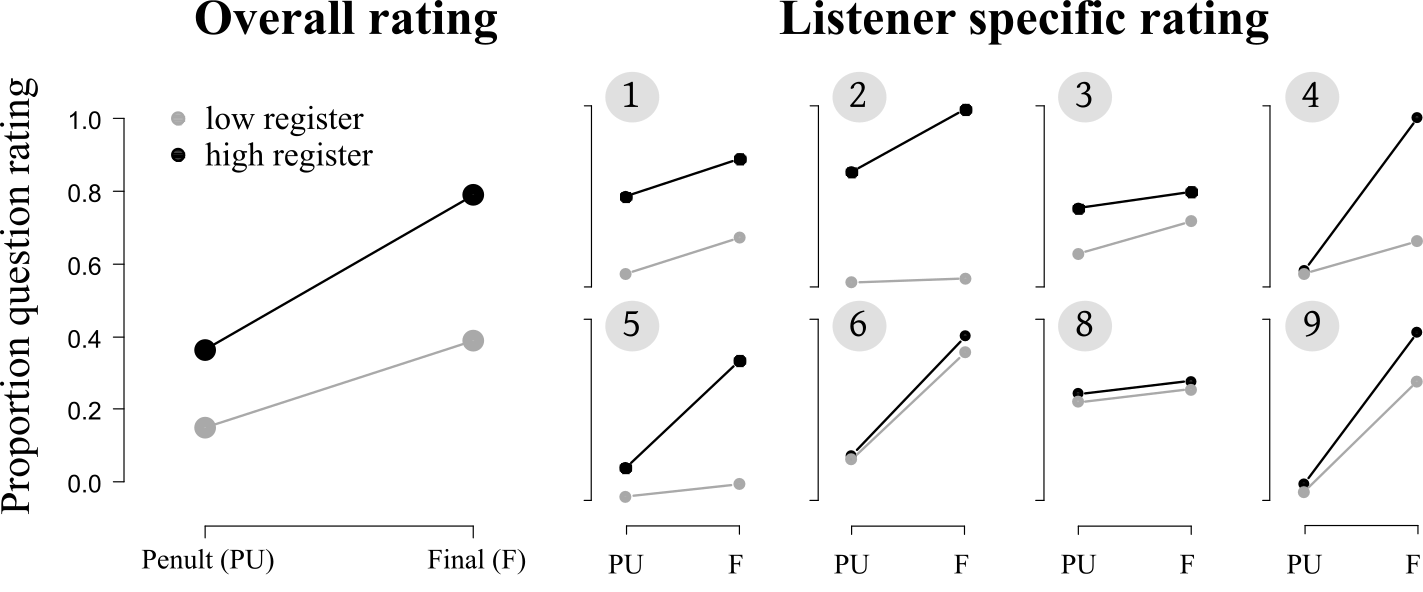
\includegraphics[width=1\textwidth]{figures/Figure_5_12.png}
  \caption{Ratings as a function of pitch register (low vs. high) and discrete peak alignment (in PU and F, respectively). Left panel displays overall results. Right panels display results for each listener individually (listener 7 was excluded as mentioned above).}
   \label{fig:5.12}
   \end{figure}

However, there appears to be no clear-cut distinction between questions and statements. Even the least preferred intonational pattern for questions (low register and pitch peak on PU) shows a considerable amount of question ratings (14\%). Even though these general trends are statistically generalisable, there is a considerable amount of variation across listeners. Consider the listener-specific patterns in \figref{fig:5.12} (right panels). Most listeners show a clear bias towards rating the high register condition as more likely to be a question (black lines are above the grey lines). In fact, some listeners show almost no question ratings when the register is low (listeners 2 and 5). Listeners 6, 8, and 9, however, seem to show a much weaker effect of pitch register. With regard to timing differences, most listeners show a clear bias towards rating sentences with the pitch peak aligned within the final syllable more likely to be a question than statements. Some listeners show almost no question ratings for pitch peaks aligned with the penult and, conversely, almost no statement ratings for pitch peaks aligned with the final syllable (listeners 4, 5, and 9). This effect appears to interact with register: the preference for questions with a pitch peak in the final syllable is stronger for the high register condition, as is very clearly illustrated by the patterns displayed by listeners 2, 4, and 5.\is{pitch scaling}\is{tonal alignment}

\largerpage
To sum up, two main factors are identified that affect the perception of morphosyntactically ambiguous sentences. First, contours in a high pitch register are perceived more frequently as questions than contours in a low register. This matches the strong pitch register differences found in the production study discussed in \sectref{sec:5.4}. Second, contours with pitch peaks on the final syllable are perceived more frequently as questions than contours with pitch peaks on the penult. However, even contours with a pitch peak on the penult appear to be acceptable contours for questions, reflecting the variation in pitch peak placement found in the production experiment. More gradual differences in tonal alignment within the syllable did not affect ratings. This null result could be due to the nature of the experimental design. Since both pitch register and discrete alignment are perceptually very prominent and represent sufficient cues to perform the task, listeners may not pay attention to subtle alignment differences. The present results are clear evidence for the rather discrete nature of peak alignment in our data. The relative peak delay is not as relevant as the position of the peak in a particular syllable.\is{pitch scaling}\is{tonal alignment}

As has been acknowledged, the low pitch target preceding the peak was set at the offset of /inna/, and the low pitch target after the peak was set to the end of the utterance. This alignment results in asymmetries in the steepness of rises and falls, across alignment conditions, with shallow rises and steep falls in peaks on the final syllable and steep rises and shallow falls in peaks on the penult. This potentially confounds the manipulation of the actual peak position (cf. \figref{fig:5.11}). Thus, the results could be interpreted as shallow rises and steep falls being more likely to be interpreted as questions than steep rises and shallow falls. The present investigation cannot rule out that the shape of the rise-fall affects listener ratings, but there are two arguments counter to this interpretation. This interpretation is not in line with the production results: rises in questions are consistently produced with substantially larger pitch excursions than statements. At the same time, the rise in pitch appears to start roughly at the same time across questions and statements. Taken together, these patterns result in substantially steeper rises in questions than in statements. Moreover, since falls are frequently truncated, the perceptual relevance of the fall is generally questionable.

\largerpage
\section{Summary}\label{sec:5.7}
The present chapter has explored the acoustic parameters associated with the distinction between contrastive statements and questions on the one hand, and information-requesting y/n questions and confirmation-seeking echo questions on the other. Production data revealed that, compared to statements, questions (a) had a higher pitch level and a greater pitch range, and (b) were more often realised with the pitch peak on the final syllable. In statements, the pitch peak occurred more often on the penult. Furthermore, there was a tendency for (c) the pitch peak in questions to be realised later within the syllable than in statements. Comparing questions types, echo questions were found to have a lower pitch level than y/n questions and a higher pitch level than corresponding statements. Other than that, the two question types revealed comparable pitch ranges and comparable peak alignment patterns.\is{pitch scaling}\is{tonal alignment}\is{focus}\is{yes-no question}\is{echo question}

The pitch register differences were consistent within and across speakers and appear to be a robust cue for disambiguating questions from statements, in both production and perception. In terms of pitch peak alignment there was a significant difference across sentence modalities in production. The perception results showed that listeners use pitch peak alignment in discrete terms (i.e. syllable-based alignment) to guide their perception of sentence modality, although pitch peaks in both syllable positions (on penult or final syllable) are acceptable locations for the pitch peak in both questions and statements.\is{tonal alignment} 

Apart from this systematic correlation of tonal placement and sentence modality, there was considerable variation in peak alignment, both within and across speakers. Additional evidence presented by \citet{Grice.etal2015tash} revealed that lexically determined segmental factors such as syllable weight of the final syllable and the sonority of syllable nuclei were relevant determinants of tonal placement. The investigated tones prefer to be realised on heavy syllables and sonorous elements. While syllables in other languages such as German or English usually contain at least a sonorant consonant, Tashlhiyt allows any type of segment in syllable nucleus position. The question arises as to how tones align with the segmental material when there are no sonorants available in the tone bearing word. The following chapter will explore these cases in detail.\is{syllable weight}\il{English}\il{German}
